\chapter{Evaluation}
\label{ch:Evaluation}
This chapter aims to validate the hypotheses formulated for two distinct studies described in Chapter~\ref{ch:Design}. 
Each study focuses on specific aspects of ear-based temperature measurement and aims to explore the capabilities and limitations of the developed wearable prototype. 
For each study, a series of hypotheses have been put forward, and the data collected from the studies are used to evaluate these hypotheses.

\section{Results and Discussion of Study 1}
\label{sec:Evaluation:Study1}
Study 1 focuses on exploring the potential and limitations of the developed ear-based temperature measurement system and examines its accuracy, reliability, and robustness under various conditions. 
A more detailed discussion of the design and objectives of Study 1 is described in Chapter~\ref{ch:Design:Study:Study1}.
Additionally, a visual representation of the procedure of Study 1 can be seen in Figure~\ref{fig:design:study1:procedure}.

Figure~\ref{fig:ch:Evaluation:Study1:RawData} shows a sample measurement from Participant 7.
The progression of slightly smoothed raw data across phases that can be seen is very similar to that of the other subjects. 
The background color represents the phase the measurement is in.
At the beginning in the acclimation phase (ID=1), the sensor adapts to the body. 
Subsequently, in the baseline phase (ID=2), the sensor readings show little change under controlled conditions.
In Phase 3, where the subjects were walking outside, the measured temperature drops for all subjects.
In the relaxation phase (ID=4), the subject is back in the controlled environment and the signal settles back toward the values measured in Phase 2.

After the study was conducted, a questionnaire was completed by each subject. 
This included the conditions and perceptions of the study. 
The study was conducted at a mean indoor temperature of $25.4 ^\circ C$ and humidity of $47.55 \text{g/m}^3$. 
The outdoor temperature was a mean of $19.375 ^\circ C$.
The external conditions were mostly sunny and cloudy, but two subjects also experienced light rain.
Subjects averaged 26 years of age (24-29) and were healthy.
All test persons arrived in such a way that they had a short journey and had not previously done any activities that could significantly influence the temperature.
After the study, all subjects were very positive about the prototype and rated it $8.1$ on a scale of 0-10.

To verify the findings collected in this study, several hypotheses were formulated and tested. 
These hypotheses aim to answer specific questions related to the performance and reliability of ear-based temperature measurements. 
The results and their implications are discussed in the following sections, where each hypothesis is evaluated in detail based on the data collected.

For proving the hypothesis to be right or wrong, t-tests are used.
The t-test is a fundamental concept in statistical hypothesis testing and shows whether two sets of data are significantly different from each other. 
It is particularly useful when small sample sizes are involved and the standard deviation of the population is unknown.
The underlying principle of the t-test is to compare the means of two groups and evaluate how likely it is that the observed differences are due to chance.
The formula for the t-statistic in an independent t-test is as follows.

\[
t = \frac{{\bar{x}_1 - \bar{x}_2}}{\sqrt{\frac{{s_1^2}}{n_1} + \frac{{s_2^2}}{n_2}}},
\]

where \( \bar{x}_1 \) and \( \bar{x}_2 \) are the sample means, \( s_1^2 \) and \( s_2^2 \) are the sample variances, and \( n_1 \) and \( n_2 \) are the sample sizes for the two groups.
The calculated t-statistic is then compared to a critical value determined by the degrees of freedom and the chosen significance level, commonly denoted by \( \alpha \).

The p-value, another important metric, quantifies the probability of obtaining the observed results if the null hypothesis were true.
The null hypothesis ($H_0$) states that the data are not significantly different when the hypothesis states that data are significantly different.
Thus, $H_0$ contradicts the hypothesis itself.
Rejecting $H_0$ further supports the hypothesis proper.
A low p-value (\( p < \alpha \)) indicates strong evidence against $H_0$, so it is rejected in favor of the alternative hypothesis.
Conversely, a high p-value indicates that the observed data are consistent with the null hypothesis.
The choice of significance level \( \alpha \), often set at 0.05, is critical because it controls the rate of type I errors that occur when a true null hypothesis is falsely rejected.

\begin{figure}[!t]
    \centering
    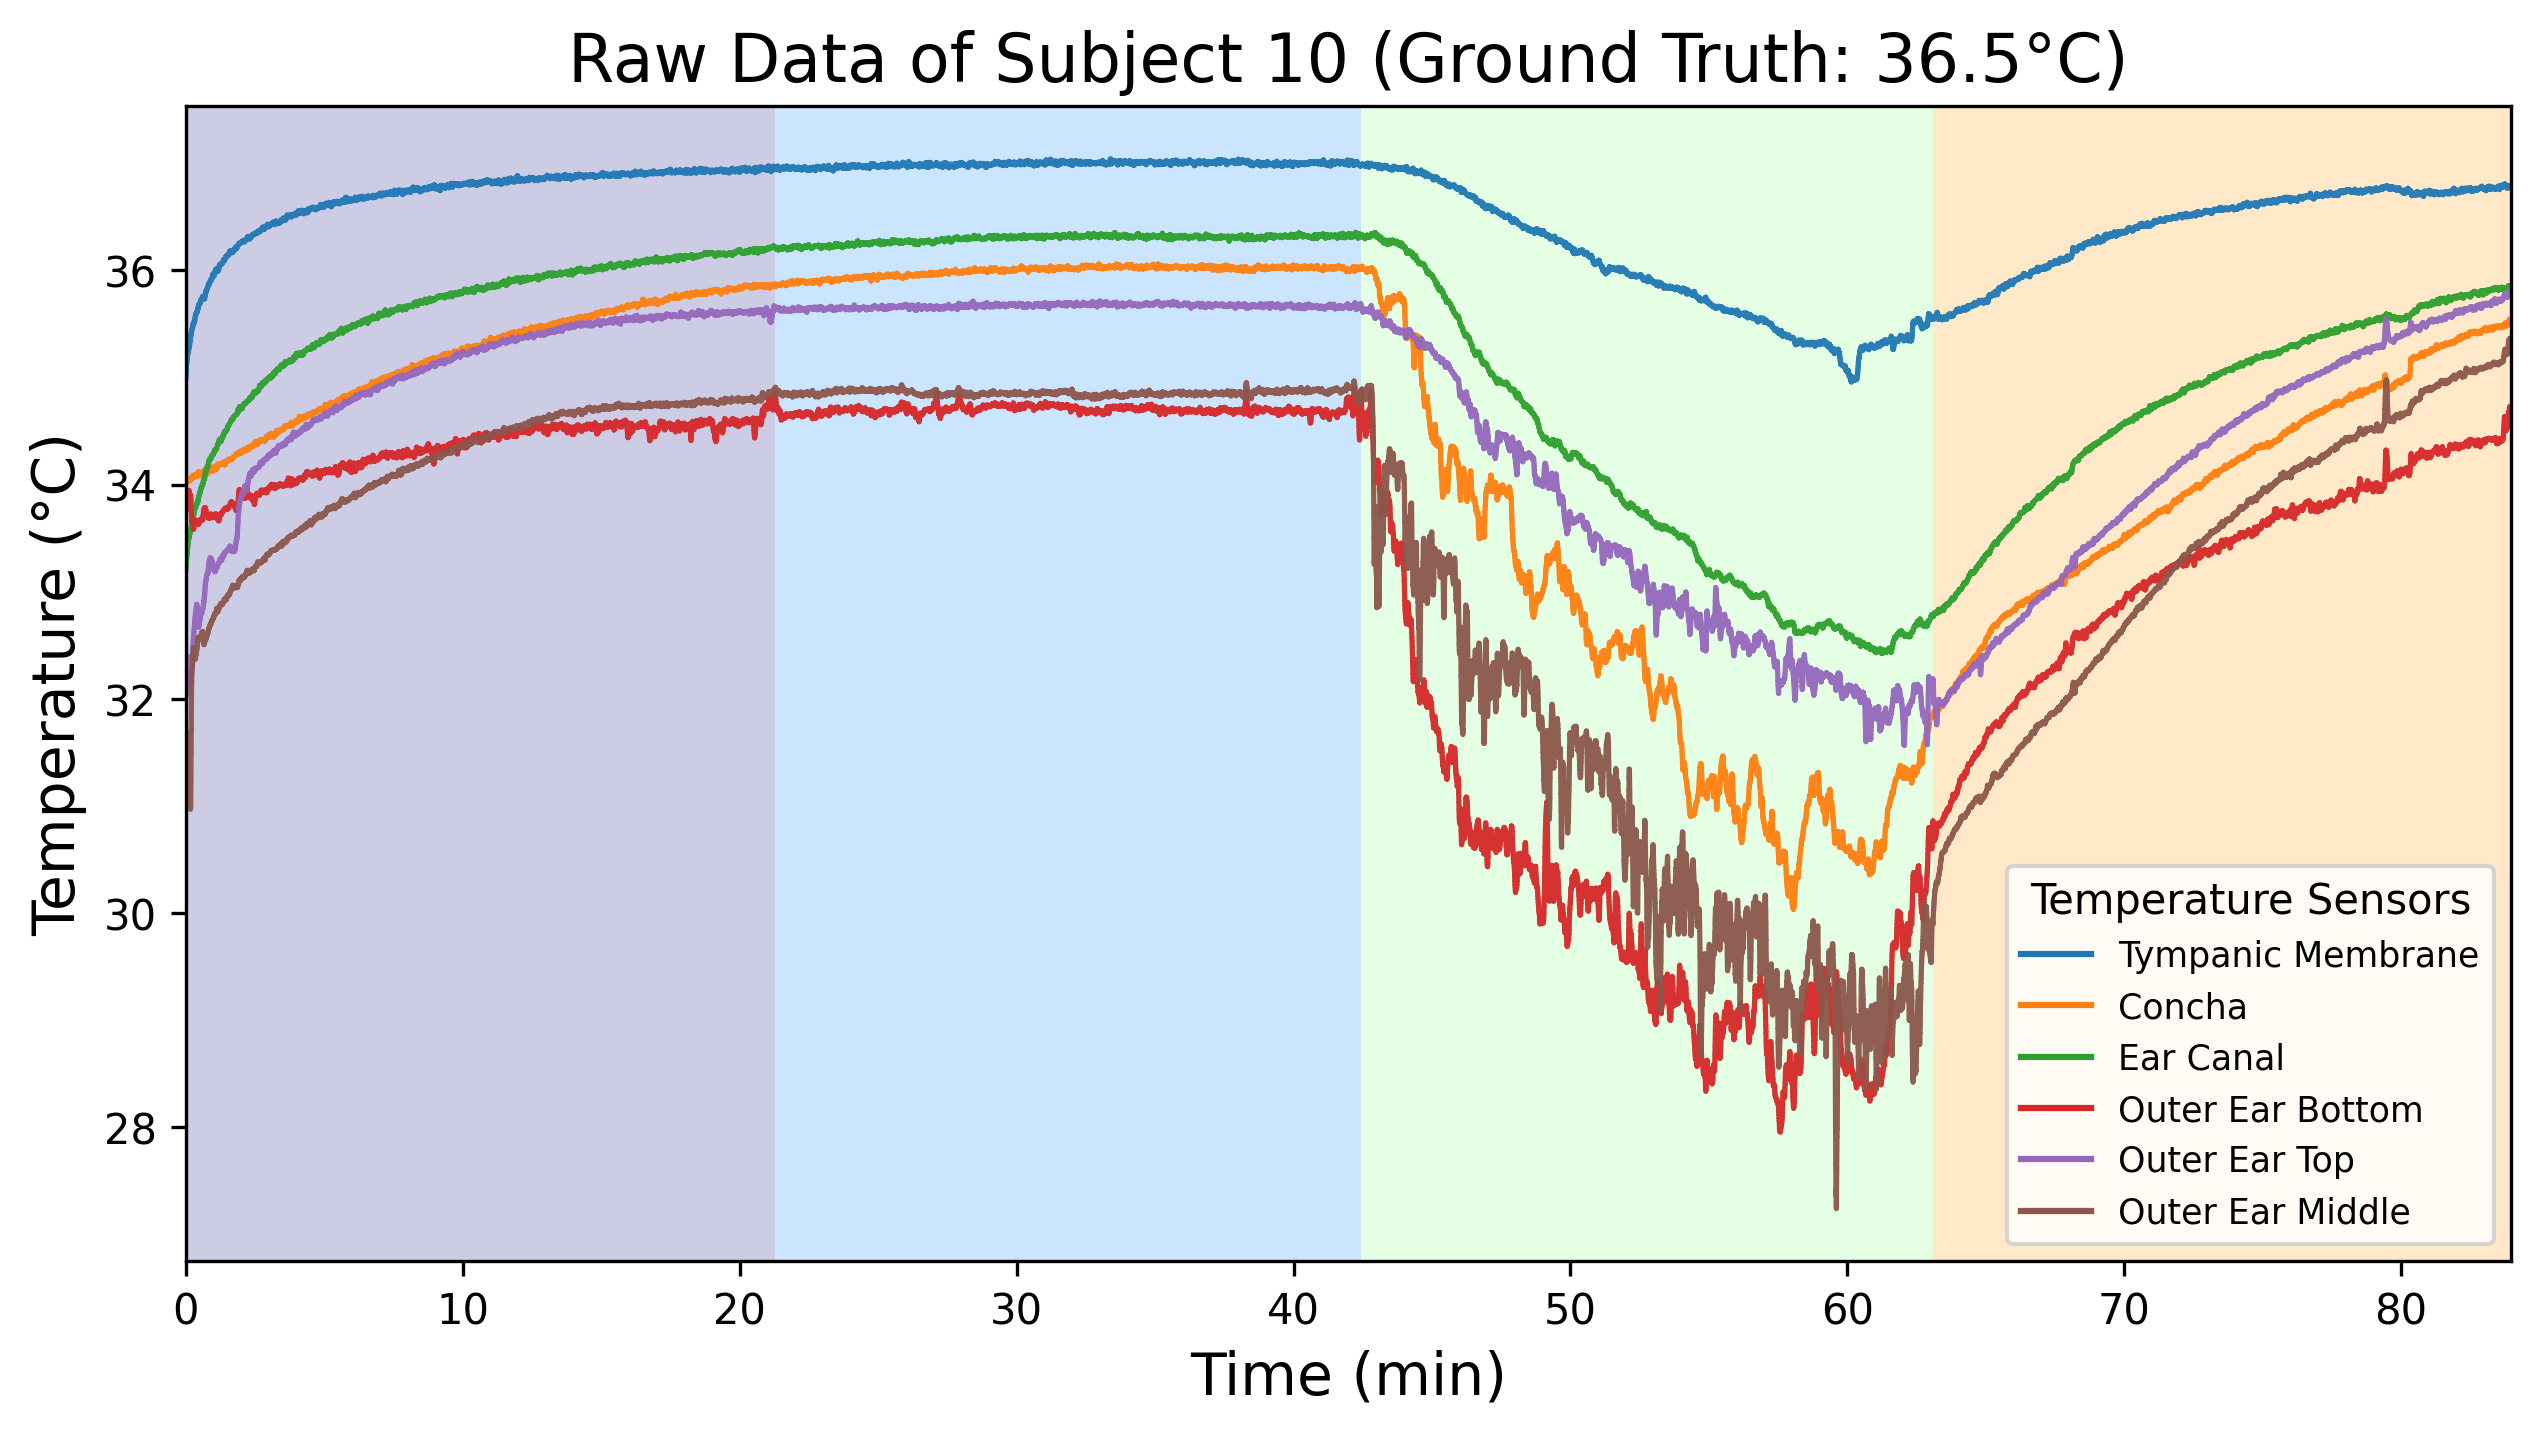
\includegraphics[width=\textwidth]{thesis-doc/images/study1/Logging_person_10_0smoothed_raw_data.png}
    \caption{Raw data of a measurement in Study 1 of Subject 10. The subject had a body temperature of $36.5^\circ\text{C}$ at the beginning. Phases 1-4 are shown, distinguished by the background color of the plot. In Phase 1, the sensor has adjusted and acclimated to the temperature of the subject. After the sensor settled in, Phase 2 measured the temperature while sitting in a room. In Phase 3, the subject went for a walk outside. In Phase 4, he went back into the room to see how the sensors settled back to the calmer environmental conditions. During the measurement, the subject was sitting on a chair in a room with closed windows. The ground truth is measured before and after the whole measurement in the same ear (right) where the prototype is placed. Also the room temperature, humidity and outdoor temperature was noted manually to complete the dataset.}
    \label{fig:ch:Evaluation:Study1:RawData}
\end{figure}

\subsection{Hypothesis 1: Lower Temperature Measured on Sensors Behind the Ear}
\label{subsec:Evaluation:Study1:Hypothesis1}

The first hypothesis is to show that a lower temperature is measured behind the ear than in the ear.
For this purpose, the analysis was considered from two points of view. 
First, only the data points where the subject was sitting were recorded, and second, all data except for the acclimatization phase (Phase 1) were considered.
In both views, a distinction was made between the two two sensor groups behind the ear (Outer Ear Top, Outer Ear Middle, Outer Ear Bottom) and in the ear (Tympanic Membrane, Ear Canal, Concha). 

In the first perspective, the data were considered when the subject was sitting (phase 2). 
Here, for all subjects, the mean temperature behind the ear was \(36.30^\circ\text{C}\), while the mean temperature inside the ear was \(36.74^\circ\text{C}\). 
To demonstrate a statistically significant difference between the two means, a t-test can be used.
This tests the probability of the null hypothesis.
The t-test yielded a p-value of \(0.0424\), which is less than the alpha value of \(0.05\). 
Thus, the null hypothesis, which states that the data are not significantly different, is true at less than $5\%$, confirming significance.
The mean error between the ground truth and the temperature measured behind the ear was \(0.50^\circ\text{C}\), and that for the temperature in the ear was \(0.18^\circ\text{C}\). 
The p-value for the comparison of these errors was \(0.0115\), again indicating a statistically significant difference.
Thus, it is clear that temperature is measured significantly lower behind the ear than in the ear while sitting.

The second perspective now also looks at other phases of the study. 
Now, in addition to the sitting phase (Phase 2), the walking phase (Phase 3) and the relaxation phase (Phase 4) were also considered. 
The mean temperature behind the ear was \(35.33^\circ\text{C}\) and in the ear it was \(36.02^\circ\text{C}\). 
The p-value of the t-test was \(0.0158\), which again is statistically significant.
The mean error behind the ear was \(1.45^\circ\text{C}\) and in the ear it was \(0.77^\circ\text{C}\). 
The p-value for the comparison of these errors was \(0.0042\), which is also statistically significant.
Thus, both perspectives support the hypothesis, both in the sitting phase only and during all activities except the acclimatization phase.

\begin{figure}[!ht]
    \centering
    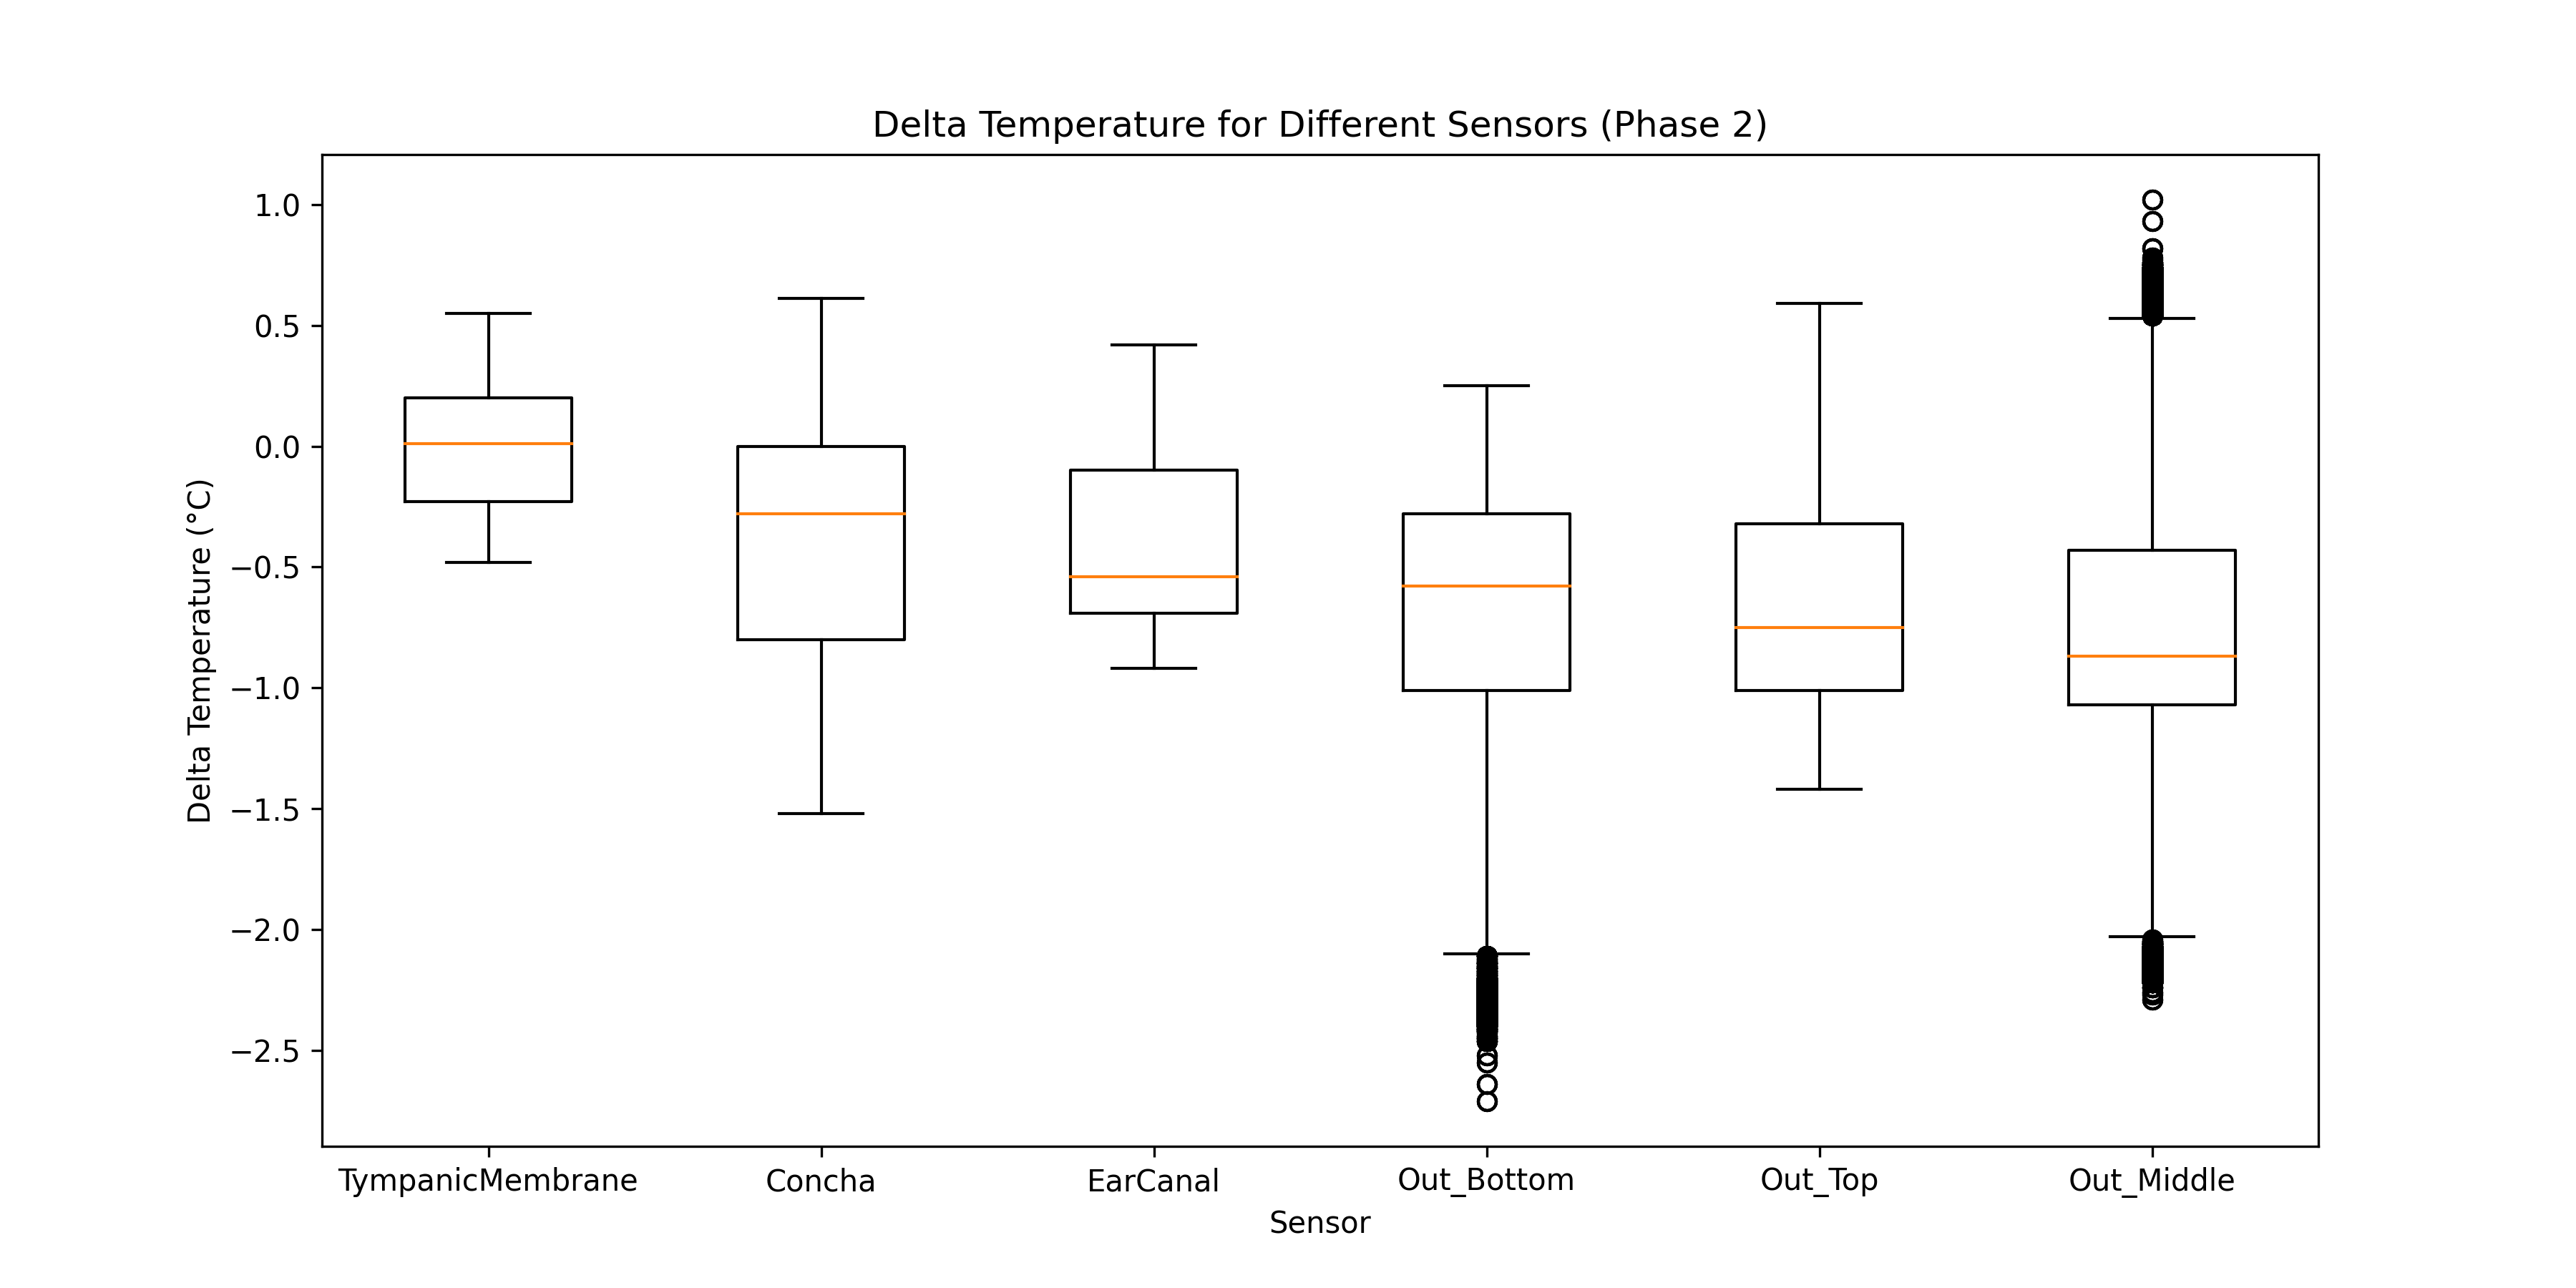
\includegraphics[width=\textwidth]{thesis-doc/images/study1/hypothesis1/hypothesis1_boxplot_phase_2.png}
    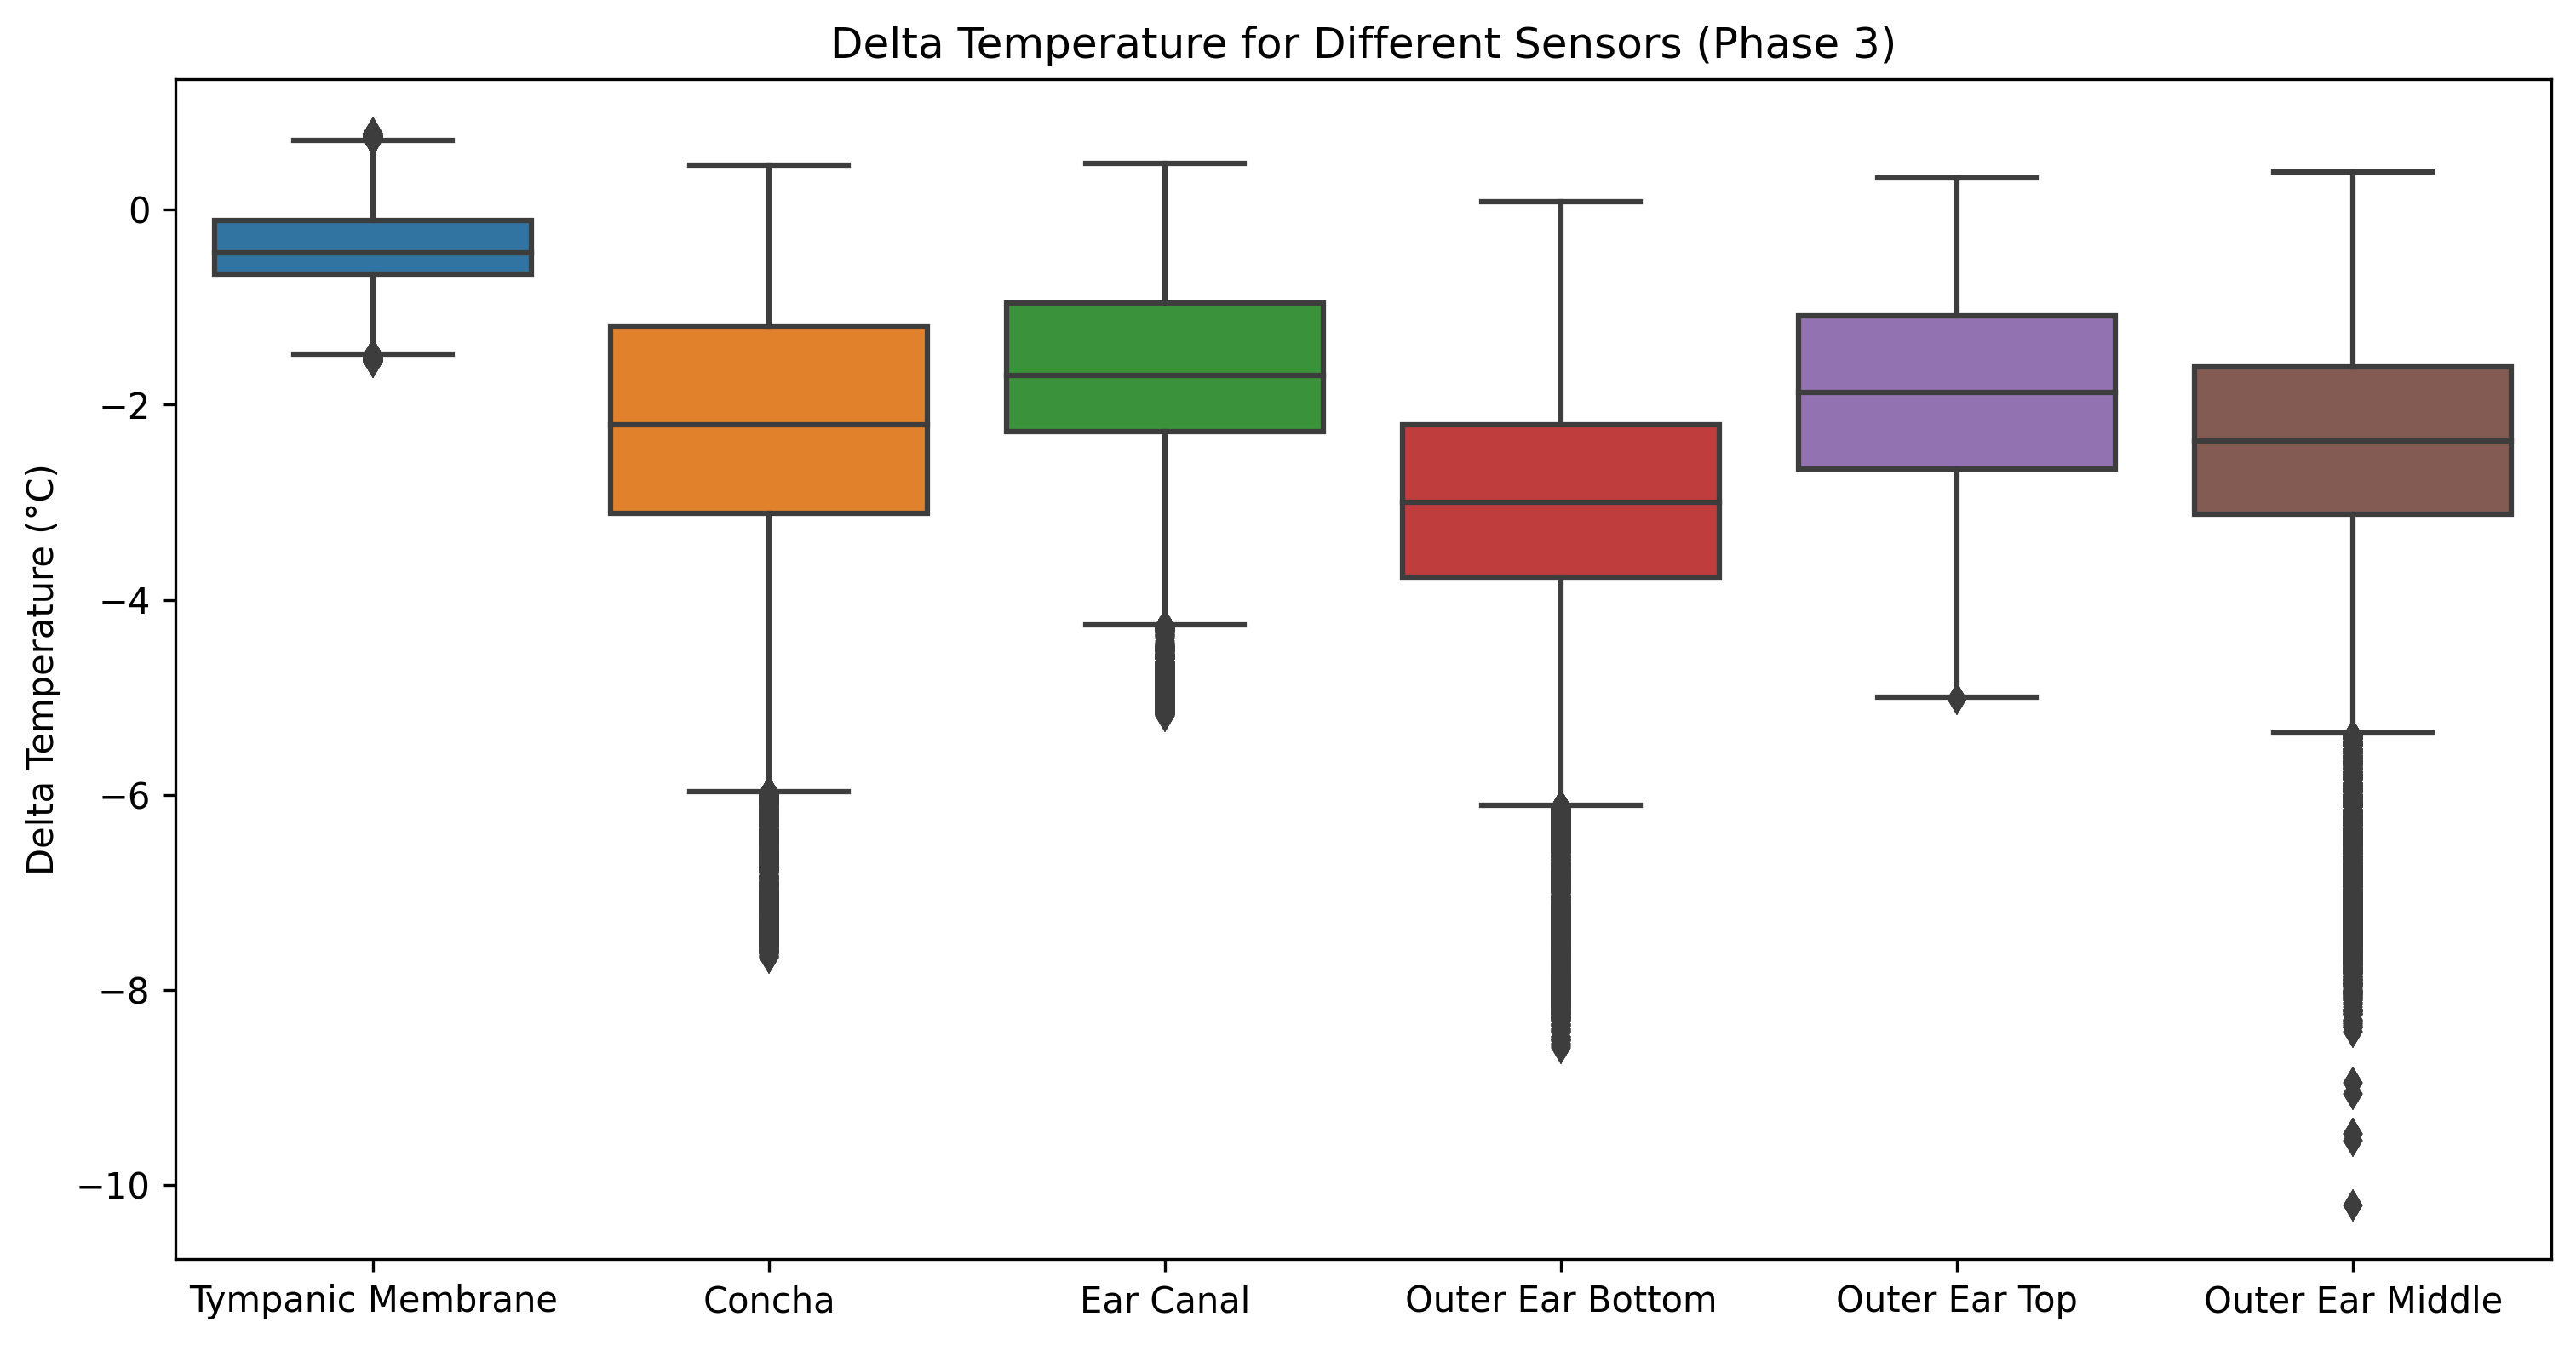
\includegraphics[width=\textwidth]{thesis-doc/images/study1/hypothesis1/hypothesis1_boxplot_phase_3.png}
    \caption{Boxplots to visually illustrate the distribution of readings from different sensor positions during Phase 2 (sitting indoors) and Phase 3 (walking outdoors). Central tendencies and their dispersion for the analysis of the sensors under different environments can be seen. Temperature values were subtracted from actual thermometer readings (ground truth) to compare all user data. These visualizations are an essential part of the evaluation of Hypotheses 1 and 2, as they highlight differences in mean temperature and variance, and highlight potential outliers.}
    \label{fig:eval:study1:hypothesis1_result}
\end{figure}

This can also be seen in Figure \ref{fig:eval:study1:hypothesis1_result}.
The two boxplot images show the sitting and walking phases (Phase 2 and 3), always zeroed to the temperature measured by the thermometer before the measurement.
During sitting (Phase 2), the temperature measured at the tympanic membrane is very close to the temperature measured by the thermometer ($\pm0.5^\circ\text{C}$). 
The sensors in the ear canal and concha also show high accuracy. 
For the sensors behind the ear, although the median is sometimes very close to the sensors in the ear, the outliers are strongly represented here, which questions the reliability of the signals.
When comparing the sensors behind the ear, the sensor placed at the top behind the ear provides the best results. 
This is due to the position behind the ear: the further below the ear, the more external influences are felt, such as a gust of wind, even if only with slight movements.
This can be seen more clearly in the boxplot for Phase 3, while the test subjects were out walking. 
While here also the sensor pointing to the tympanic membrane shows the best results, all other sensors have outliers.
There is also a significant difference between the sensor in the ear canal and the auricle. 
The sensor in the ear canal is further in the ear and thus somewhat more protected from external conditions, which is also evident here. 
The findings of the boxplot from Phase 2 are also confirmed for the sensors behind the ear.

The second perspective, which uses Phase 2,3 and 4 also confirms the hypothesis that the temperature measured behind the ear is statistically significantly lower than that measured in the ear. 
However, the sensors behind the ear also show a statistically significant higher error compared to the ground truth, especially when the subject is involved in activities such as walking. 
These findings have important implications for the use of ear-based temperature sensors in various applications.

\subsection{Hypothesis 2: Indoor vs Outdoor Variance}
\label{subsec:Evaluation:Study2:Hypothesis2}

\begin{table}[t]
\centering
\begin{tabular}{|p{2.5cm}|c|c|c|c|c|c|}
\hline
\textbf{Sensor} & \multicolumn{2}{c|}{\textbf{MAD}} & \multicolumn{2}{c|}{\textbf{Mean Variance}} & \multicolumn{2}{c|}{\textbf{Mean Diff. from}} \\
 & \multicolumn{2}{c|}{\textbf{(in \(^\circ\text{C}\))}} & \multicolumn{2}{c|}{\textbf{(in \(^\circ\text{C}^2\))}} & \multicolumn{2}{c|}{\textbf{Ground Truth (in \(^\circ\text{C}\))}} \\
\hline
 & \textbf{Indoor} & \textbf{Outdoor} & \textbf{Indoor} & \textbf{Outdoor} & \textbf{Indoor} & \textbf{Outdoor} \\
\hline
\textbf{Tympanic Membrane} & 0.025 & 0.258 & 0.00097 & 0.107 & 0.224 & -0.391 \\
\textbf{Concha} & 0.042 & 0.820 & 0.00307 & 1.134 & -0.164 & -2.344 \\
\textbf{EarCanal} & 0.030 & 0.624 & 0.00155 & 0.646 & -0.177 & -1.742 \\
\textbf{O.E. Bottom} & 0.095 & 0.800 & 0.01890 & 1.110 & -0.527 & -3.094 \\
\textbf{O.E. Top} & 0.062 & 0.663 & 0.00694 & 0.650 & -0.389 & -1.903 \\
\textbf{O.E. Middle} & 0.101 & 0.831 & 0.01980 & 1.098 & -0.529 & -2.548 \\
\hline
\end{tabular}
\caption{Mean absolute deviation (MAD), mean variance, and mean distance from ground truth for different sensors (O.E. = Outer Ear). Phases 2 (inside) and 3 (outside) were considered. All values were calculated for each sensor and averaged over all subjects.}
\label{subsec:Evaluation:Study1:Hypothesis2:mean_variance_table}
\end{table}

The second hypothesis is to show that the variance in temperature readings from ear-based sensors is lower indoors than outdoors.
This expectation is derived from the fact that the external influences in an indoor environment with closed windows are significantly less than the external influences outside during walking.
To test this hypothesis empirically, the data set of several ear-based temperature sensors at different positions was considered, both indoors and outdoors.
The different situations within the studies were divided into phases. 
Phase 2 represents an indoor measurement and Phase 3 represents an outdoor measurement during walking.
Here, the temperature values in different areas of the ear were looked at closely.
To prove the hypothesis, the variances per temperature sensor were now calculated for phases 2 and 3 respectively. 
The results show a clear pattern. 
The mean variance for the tympanic membrane sensor is $0.00097$ indoors and $0.1074$ outdoors.
This pattern was consistently observed for other sensor locations, such as the concha with a mean variance of $0.00307$ indoors and $1.134$ outdoors.
A detailed listing of the results can be seen in Table \ref{subsec:Evaluation:Study1:Hypothesis2:mean_variance_table}.

\begin{table}[h]
\centering
\begin{tabularx}{\textwidth}{|X|c|}
\hline
\textbf{Sensor} & \textbf{p-value} \\
\hline
Tympanic Membrane & \(0.0005438\) \\
Concha & \(0.0005870\) \\
Ear Canal & \(0.0005009\) \\
Outer Ear Bottom & \(4.71 \times 10^{-6}\) \\
Outer Ear Top & \(7.04 \times 10^{-7}\) \\
Outer Ear Middle & \(0.0002436\) \\
\hline
\end{tabularx}
\caption{P-values from the Bonferroni-corrected t-tests of the different sensors using the indoor and outdoor variances.}
\label{subsec:Evaluation:Study1:Hypothesis2:pvalues}
\end{table}

To test this hypothesis, the variances of each sensor's temperature readings were calculated for both the indoor (Phase 2) and outdoor (Phase 3) situations.
A two-sample t-test was then applied to statistically compare these variances for each sensor.
Because multiple comparisons were made for different sensors, a Bonferroni correction was applied to control for the family-specific error rate.
The Bonferroni corrected threshold was used to determine the statistical significance of the results.
For example, the p-value for the tympanic membrane sensor was significantly lower than the Bonferroni-corrected threshold, allowing us to reject the null hypothesis.
This pattern was consistently observed for other sensors (see Table~\ref{subsec:Evaluation:Study1:Hypothesis2:pvalues}), providing strong empirical support for the hypothesis.
In summary, the data confirm that temperature readings from ear-based sensors have significantly lower variances when measured indoors compared to outdoors.

\subsection{Hypothesis 3: Interrelated Temperature Changes}
\label{subsec:Evaluation:Study1:Hypothesis3}
The third hypothesis examines the correlation between the relative changes in temperature readings from different sensor locations in Phases 2 and 3.
This is used to understand the consistency between the different sensor readings, especially in relation to changing weather conditions.
The mean absolute deviation (MAD) is used for analysis to better understand the consistency between the different temperature sensor readings. 
Table \ref{subsec:Evaluation:Study1:Hypothesis2:mean_variance_table} shows the MAD value for each sensor location in Phase 2 (indoor) and 3 (outdoor).

Initial trends can be seen in the mean distance to ground truth.
For example, in the outdoor phase, the temperature drops significantly compared to the indoor phase.
While the sensor measurement in Phase 2 at the tympanic membrane deviates $0.2 ^\circ\text{C}$ from ground truth, the other sensor locations have a mean change up to $-0.53^\circ\text{C}$ from ground truth.
This is seen even more strongly in the outdoor area. 
While here the measurement at the tympanic membrane deviates by $-0.391 ^\circ\text{C}$ from the ground truth, the other sensor locations have a mean change up to $-3.094^\circ\text{C}$.
This is mainly due to the fact that external influences such as wind, rain or sunlight may play a large role here.
When the test persons went for a walk, these influences occurred more often, which explains the deviations here. 
In addition, the outdoor temperature at the end of September when recorded at about $20^\circ\text{C}$ was significantly lower than the indoor temperature of about $25-27^\circ\text{C}$.
This shows that these sensor positions are not as stable to external environmental influences as the sensor directed at the tympanic membrane.
This is exactly what is shown in the mean absolute deviation. 

Mean absolute deviation (MAD) serves as a robust metric to quantify the stability of different sensor locations under varying environmental conditions. 
As shown in Table \ref{subsec:Evaluation:Study1:Hypothesis2:mean_variance_table}, the MAD values for indoor and outdoor environments differ significantly. 
For example, the tympanic sensor has a low MAD value of \(0.025 ^\circ\text{C}\) for indoor measurements, indicating that it provides very consistent readings in controlled environments. 
However, this value increases to \(0.258 ^\circ\text{C}\) in the outdoor phase, indicating increased susceptibility to environmental factors such as wind and temperature variations. 
This is consistent with the observed mean deviation from ground truth, further confirming the relevance of MAD as an assessment metric. 
Other sensors, particularly those positioned outdoors such as Outer Ear Bottom and Outer Ear Middle, also show a significant increase in MAD values as they transition from an indoor to an outdoor environment. 
This is consistent with their increased mean differences from ground truth and highlights their volatility in response to external influences. 
Thus, the MAD values illustrate the central message of this hypothesis: sensors vary in their stability in response to external environmental influences, and this variation is quantifiable.

\begin{figure}[!t]
    \centering
    % 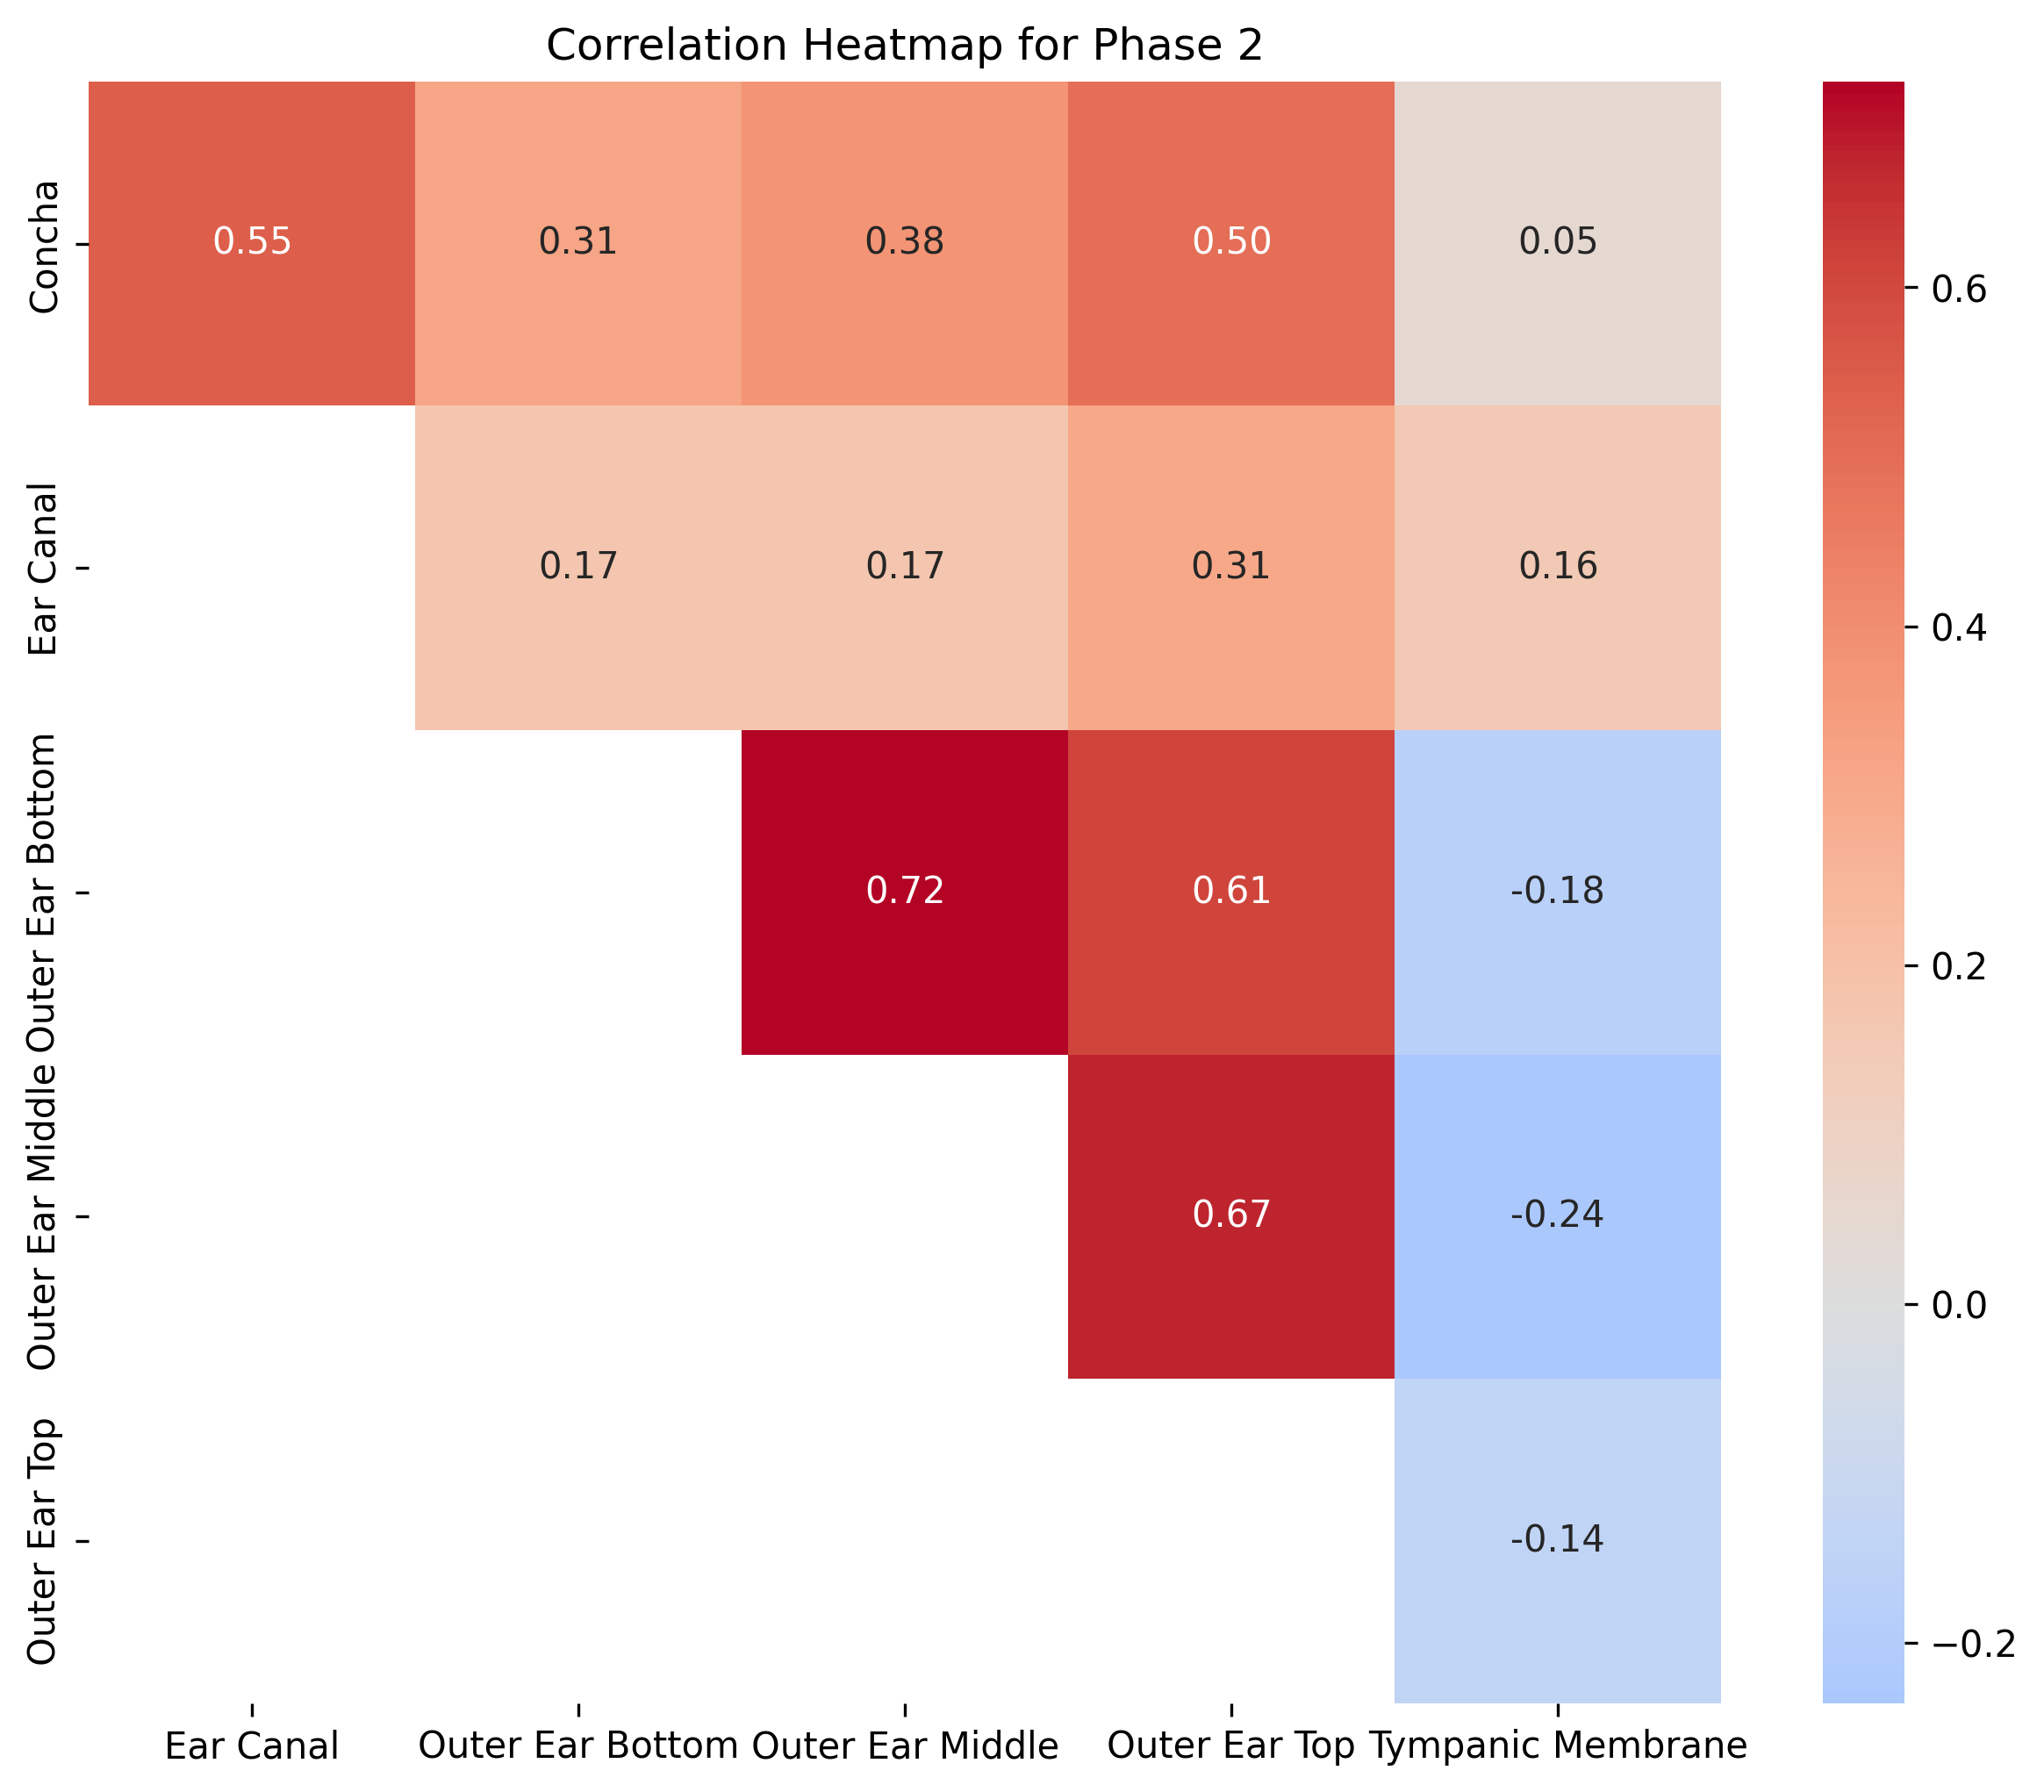
\includegraphics[width=0.75\textwidth]{thesis-doc/images/study1/hypothesis3/Correlation_Heatmap_Phase_2.png}
    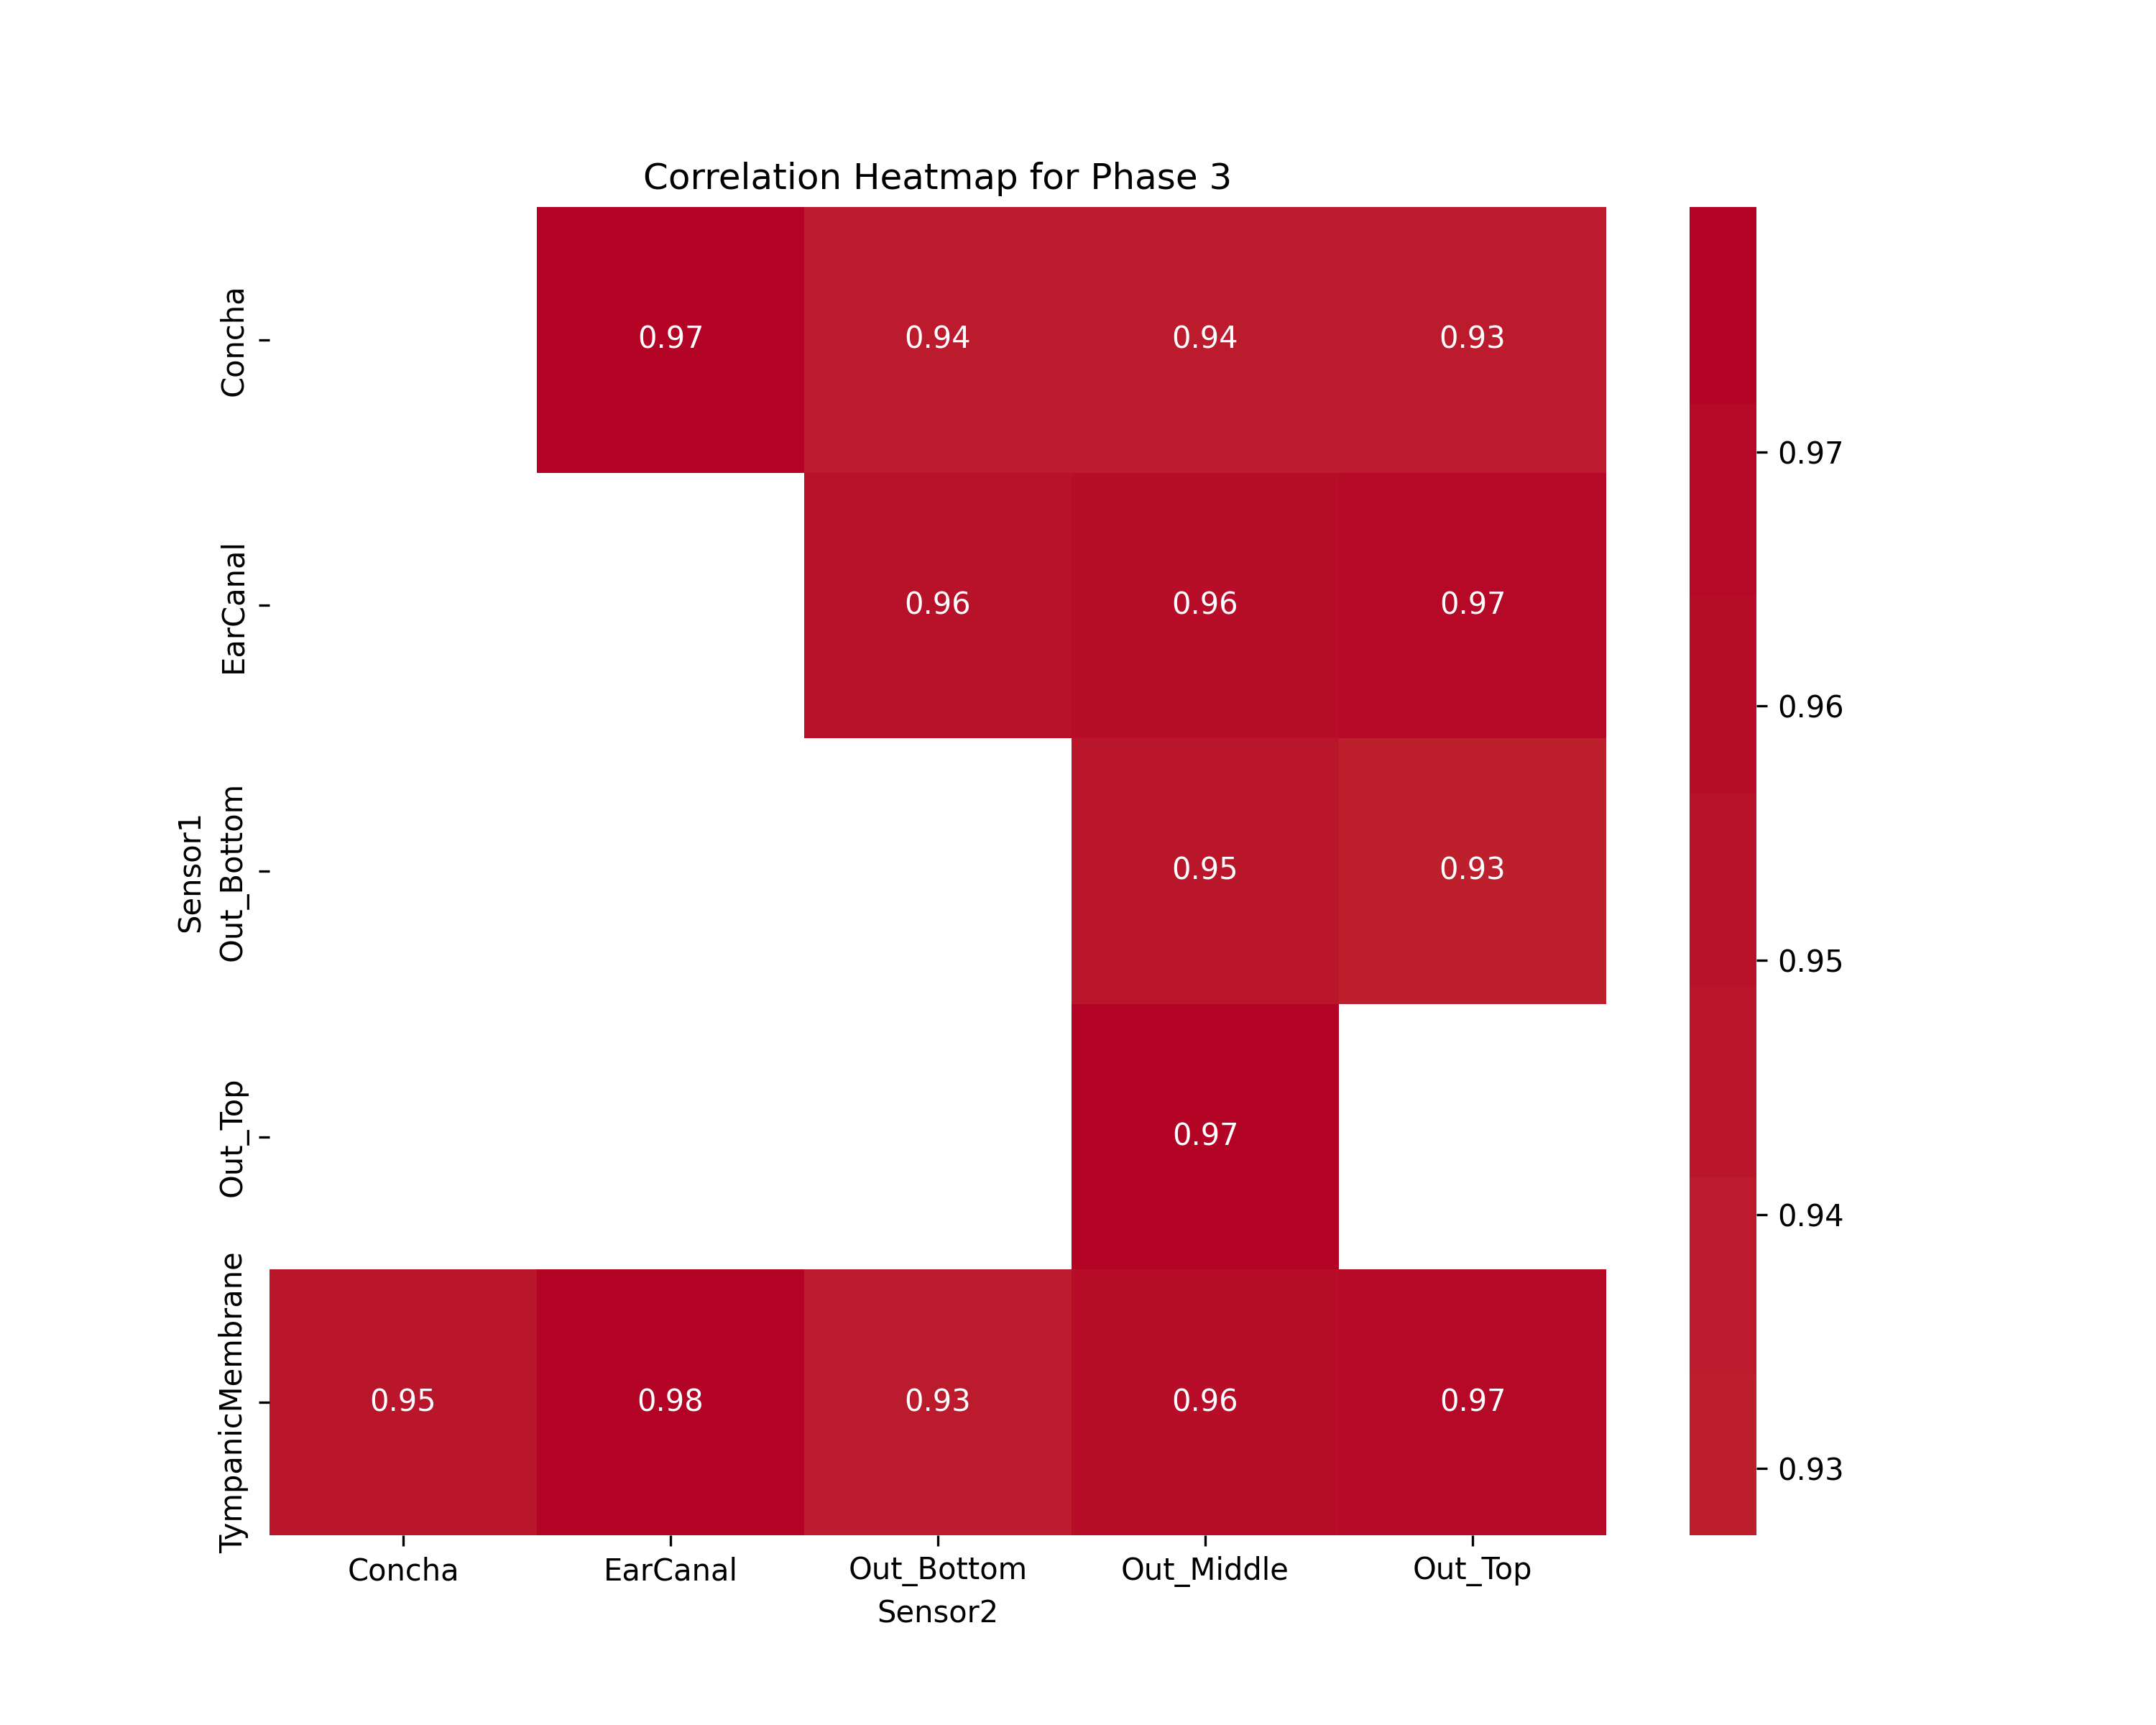
\includegraphics[width=0.75\textwidth]{thesis-doc/images/study1/hypothesis3/Correlation_Heatmap_Phase_3.png}
    \caption{Heat maps showing the Spearman correlation matrices of temperature readings from different ear-based sensors during Phase 3 (outdoor). The Spearman correlation values range from -1 to 1, where -1 indicates a perfect inverse relationship, 1 indicates a perfect direct relationship, and 0 suggests no correlation. The color-coded matrices offer a nuanced visual representation of these correlations: darker shades signify stronger positive correlations while lighter shades indicate weaker or negative correlations. These matrices not only assess the consistency between sensor measurements but also reflect their sensitivity to external environmental changes, thus providing empirical evidence for Hypothesis 3.}    
    \label{fig:eval:study1:hypothesis3_result}
\end{figure}

This can also be seen in the heatmap in Figure \ref{fig:eval:study1:hypothesis3_result}.  
Correlations between pairs of sensors are calculated using Spearman's rank correlation, which is more robust to outliers and non-linear relationships.  
% Phase 2 (interiors) shows a mixed set of correlation values, with some even showing a negative correlation, such as the pair of tympanic tubes and Outer Ear Bottom (\(r = -0.163\)).  
% This suggests that not all sensors are equally sensitive to the same factors, which could be due to individual positioning or unique interactions with environmental or physiological variables.  
Phase 3 (outdoors) shows uniformly high correlations, often above \(0.9\), across all sensor pairs.  
This suggests that the sensors behave more coherently when subjects are outdoors, possibly due to a common response to environmental factors such as wind and sunlight.  
It is noteworthy that the tympanic membrane sensor, which showed aberrant behavior indoors, closely matched the other sensors outdoors.
However, it is clearly seen here in the raw data that temperature measurements in the ear drop less than temperature measurements behind the ear. 
This is confirmed by the MAD and mean deviations to ground truth. 
Thus, the heat map not only supports the primary hypothesis, but also reveals subtleties about how each sensor responds to different conditions.
Additionally, together with the MAD and mean deviation to ground truth, it provides confirmation of the hypothesis.

In summary, the heat map supports the hypothesis by showing that indoor sensor readings fluctuate widely, while outdoor conditions tend to synchronize readings, albeit with higher volatility.
This hypothesis is supported by the analysis of the mean absolute deviation. 
Furthermore, it can be seen that the sensors at the different positions are differently stable to external environmental influences, especially when the subjects are outdoors.

\subsection{Hypothesis 4: Temperature at the Tympanic Membrane Is Most Stable}
\label{subsec:Evaluation:Study1:Hypothesis4}
The fourth hypothesis considers the stability of temperature sensor readings at the tympanic membrane compared to other positions during phases 2 (indoor) and 3 (outdoor).
The metric used here is the standard deviation. 
The standard deviation results can be found in Table \ref{subsec:Evaluation:Study1:Hypothesis4:std_dev_table}. 
In Phase 2, the standard deviation is still relatively similar for all measurements, with only the position behind the ear in the middle yielding a worse value of $0.1154$. 
The standard deviation from the tympanic membrane nevertheless sets itself apart from those of the others with $0.0288$ compared to $0.05-0.07$. 
In Phase 3, however, it is clear that the measurement of temperature at the tympanic membrane shows the most stability. 
At $0.1971$, the deviation is significantly smaller than for the rest $0.65-0.92$. 
Additionally, it can be seen from Figure \ref{fig:eval:study1:hypothesis1_result} that measurements at the tympanic membrane show the least quantile differences and are closest to the thermometer values. 
From the calculated standard deviations, it appears that the tympanic membrane has the lowest values in both phases, indicating higher stability. 
In contrast, the other sensors show higher standard deviations, more specifically the sensors outside the ear. 
This makes them more susceptible to external conditions, such as environmental changes.
Thus, this confirms the hypothesis that the tympanic membrane measurement provides the most stable temperature readings.

\begin{table}[t]
\centering
\begin{tabular}{|l|c|c|}
\hline
\textbf{Sensor} & \textbf{Mean Standard Deviation} & \textbf{Mean Standard Deviation} \\
& \textbf{Phase 2 (indoor)} & \textbf{Phase 3 (outdoor)} \\
\hline
\textbf{Tympanic Membrane} & 0.0308 & 0.3048 \\
\textbf{Concha} & 0.0535 & 0.9882 \\
\textbf{Ear Canal} & 0.0378 & 0.7496 \\
\textbf{Outer Ear Bottom} & 0.1138 & 1.0156 \\
\textbf{Outer Ear Top} & 0.0730 & 0.7836 \\
\textbf{Outer Ear Middle} & 0.1176 & 0.9875 \\
\hline
\end{tabular}
\caption{Mean Standard deviations of temperature readings for different sensors during phases 2 and 3, averaged over all subjects. Lower values indicate higher stability.}
\label{subsec:Evaluation:Study1:Hypothesis4:std_dev_table}
\end{table}

\subsection{Hypothesis 5: Movement Leads to Changes in the Temperature Readings}
\label{subsec:Evaluation:Study1:Hypothesis5}
\begin{figure}[!t]
    \centering
    \includegraphics[width=\textwidth]{thesis-doc/images/study1/hypothesis5/Hypothesis5_Analysis.png}
    \caption{Analysis of mean absolute relative change (MARC) for ear-based temperature readings and mean absolute motion. The MARC for six different sensor positions in the ear is plotted for phases 2, 3, and 4 of the study. The last subgraph shows the mean motion calculated from the IMU data during the same phases.}    
    \label{fig:eval:study1:hypothesis5_result}
\end{figure} 
Hypothesis 5 addresses the evaluation of the effect of participant movement on the variability of temperature measurements at different ear-based sensor locations.
This analysis was conducted with calibration data that included both temperature and IMU data. 
Temperature data were collected from six strategically placed sensors: Tympanic Membrane, Concha, Auditory Canal, Outer Ear Bottom, Outer Ear Top and Outer Ear Center.
A 9-axis IMU sensor was used to measure mean inertial motion. 
The analysis was limited to phases 2, 3 and 4 of the calibration procedure because Phase 1 is used to acclimate the sensors.
The mean absolute relative temperature change (MARC) was calculated for each sensor position and plotted versus time.
For this purpose, the formula:
\[
\text{relative change} = \left| T_{\text{current}} - T_{\text{previous}} \right|,
\]

was used, where \( T_{\text{current}} \) and \( T_{\text{previous}} \) are the current and previous temperature values, respectively. 

Figure \ref{fig:eval:study1:hypothesis5_result} shows the mean relative absolute changes (MARC) per sensor, averaged across all subjects.
These MARC plots per temperature sensor were combined with the mean motion data in a time series plot.
This approach effectively captures the total motion intensity at each time point by considering all available IMU sensors.
The motion data were averaged across all sensors and subjects to capture motion in all directions.
The result shows a noticeable correlation between changes in temperature readings and subject motion, a consistency observed across different sensor positions.
The temperature sensor aimed at the tympanic membrane shows the least change with movement, followed by the sensor in the ear canal.
Somewhat surprisingly, the sensor behind the concha appears to show less change than the sensor inside the concha. 
However, the other two sensors behind the ear in the middle and bottom show much stronger relative changes. 
This is likely due in part to the fact that the sensors behind the ear, which are located slightly lower and are less protected by the hair, are more sensitive to environmental influences. 
The concha is also much more exposed to environmental influences from the front, which also explains the increase in this sensor.
In general, relative changes can be seen for the individual temperature sensors in the three phases, but this may be due to different conditions. 
In Phase 3, the temperature generally decreased significantly when the subjects left the room and went outside.
This is exacerbated by exercise during the outdoor phase. 
Thus, it cannot be clearly stated whether this is due to the outdoor temperature drop, the exercise itself or both.
This evaluation provides the basis for future research on optimal sensor positioning and data fusion techniques for ear-based temperature sensing, especially during movement, but needs to be verified by further studies.

\clearpage
\section{Results and Discussion of Study 2}
\label{sec:Evaluation:Study2}
Having checked the validity of the temperature measurements, a second study will now observe how the measured temperature behaves when the subject is placed under stress.
A more detailed introduction to the design and objectives of Study 2 is described in Chapter~\ref{ch:Design:Study:Study2}.
Additionally, a visual representation of the procedure of Study 2 can be seen in Figure~\ref{fig:design:study2:procedure}.

After the study was conducted, a questionnaire was completed by each subject. 
This included the conditions and perceptions of the study. 
The study was conducted at a mean indoor temperature of $23.16 ^\circ C$ and humidity of $53.56 \text{g/m}^3$. 
The outdoor temperature averaged $20.6 ^\circ C$.
The external conditions were mostly sunny and cloudy.
Subjects averaged 26 years of age (24-29) and were healthy.
All test persons arrived in such a way that they had a short journey and had not previously done any activities that could significantly influence the temperature.
After the study, all subjects were very positive about the prototype and rated it a $7.8$ on a scale of 0-10.
In comparison to the questionnaire from the first study, a NASA-TLX questionnaire was also attached, which should make the stress of the stress-induced phase more tangible.
The scale here ranges from 0-10.
Here, the mental demand was rated on average at $7.1$, as well as the physical demand at $0.4$. 
Since the stress tests (stroop test, N-back test, math test) each have mental demands and do not require physical demands, this reflects the expectation.
Since the study was also expected to elicit time stress, the time requirement was also expected to be high.
This was confirmed with a score of $7.3$.
Since the tasks were designed to not all be solvable in time, subjects were also asked about their personal performance.
This was answered very differently, as some subjects were very satisfied with their performance, but others were not at all. 
This resulted in the mean value of $5.3$.
The effort of the subjects was on average $6.5$ and the frustration was $4.6$.

In order to fundamentally assess stress for the first time, an HRV measurement with the Polar H9 is performed in parallel.
The raw data of the study measurement on Subject 4 can be seen in Figure \ref{fig:ch:Evaluation:Study2:RawData}.
This will first test whether the subjects actually experienced stress during the study in Phase 3 by looking at the HRV signal and classifying the stress.
Hypotheses are then tested and proven or disproven.

\begin{figure}[!t]
    \centering
    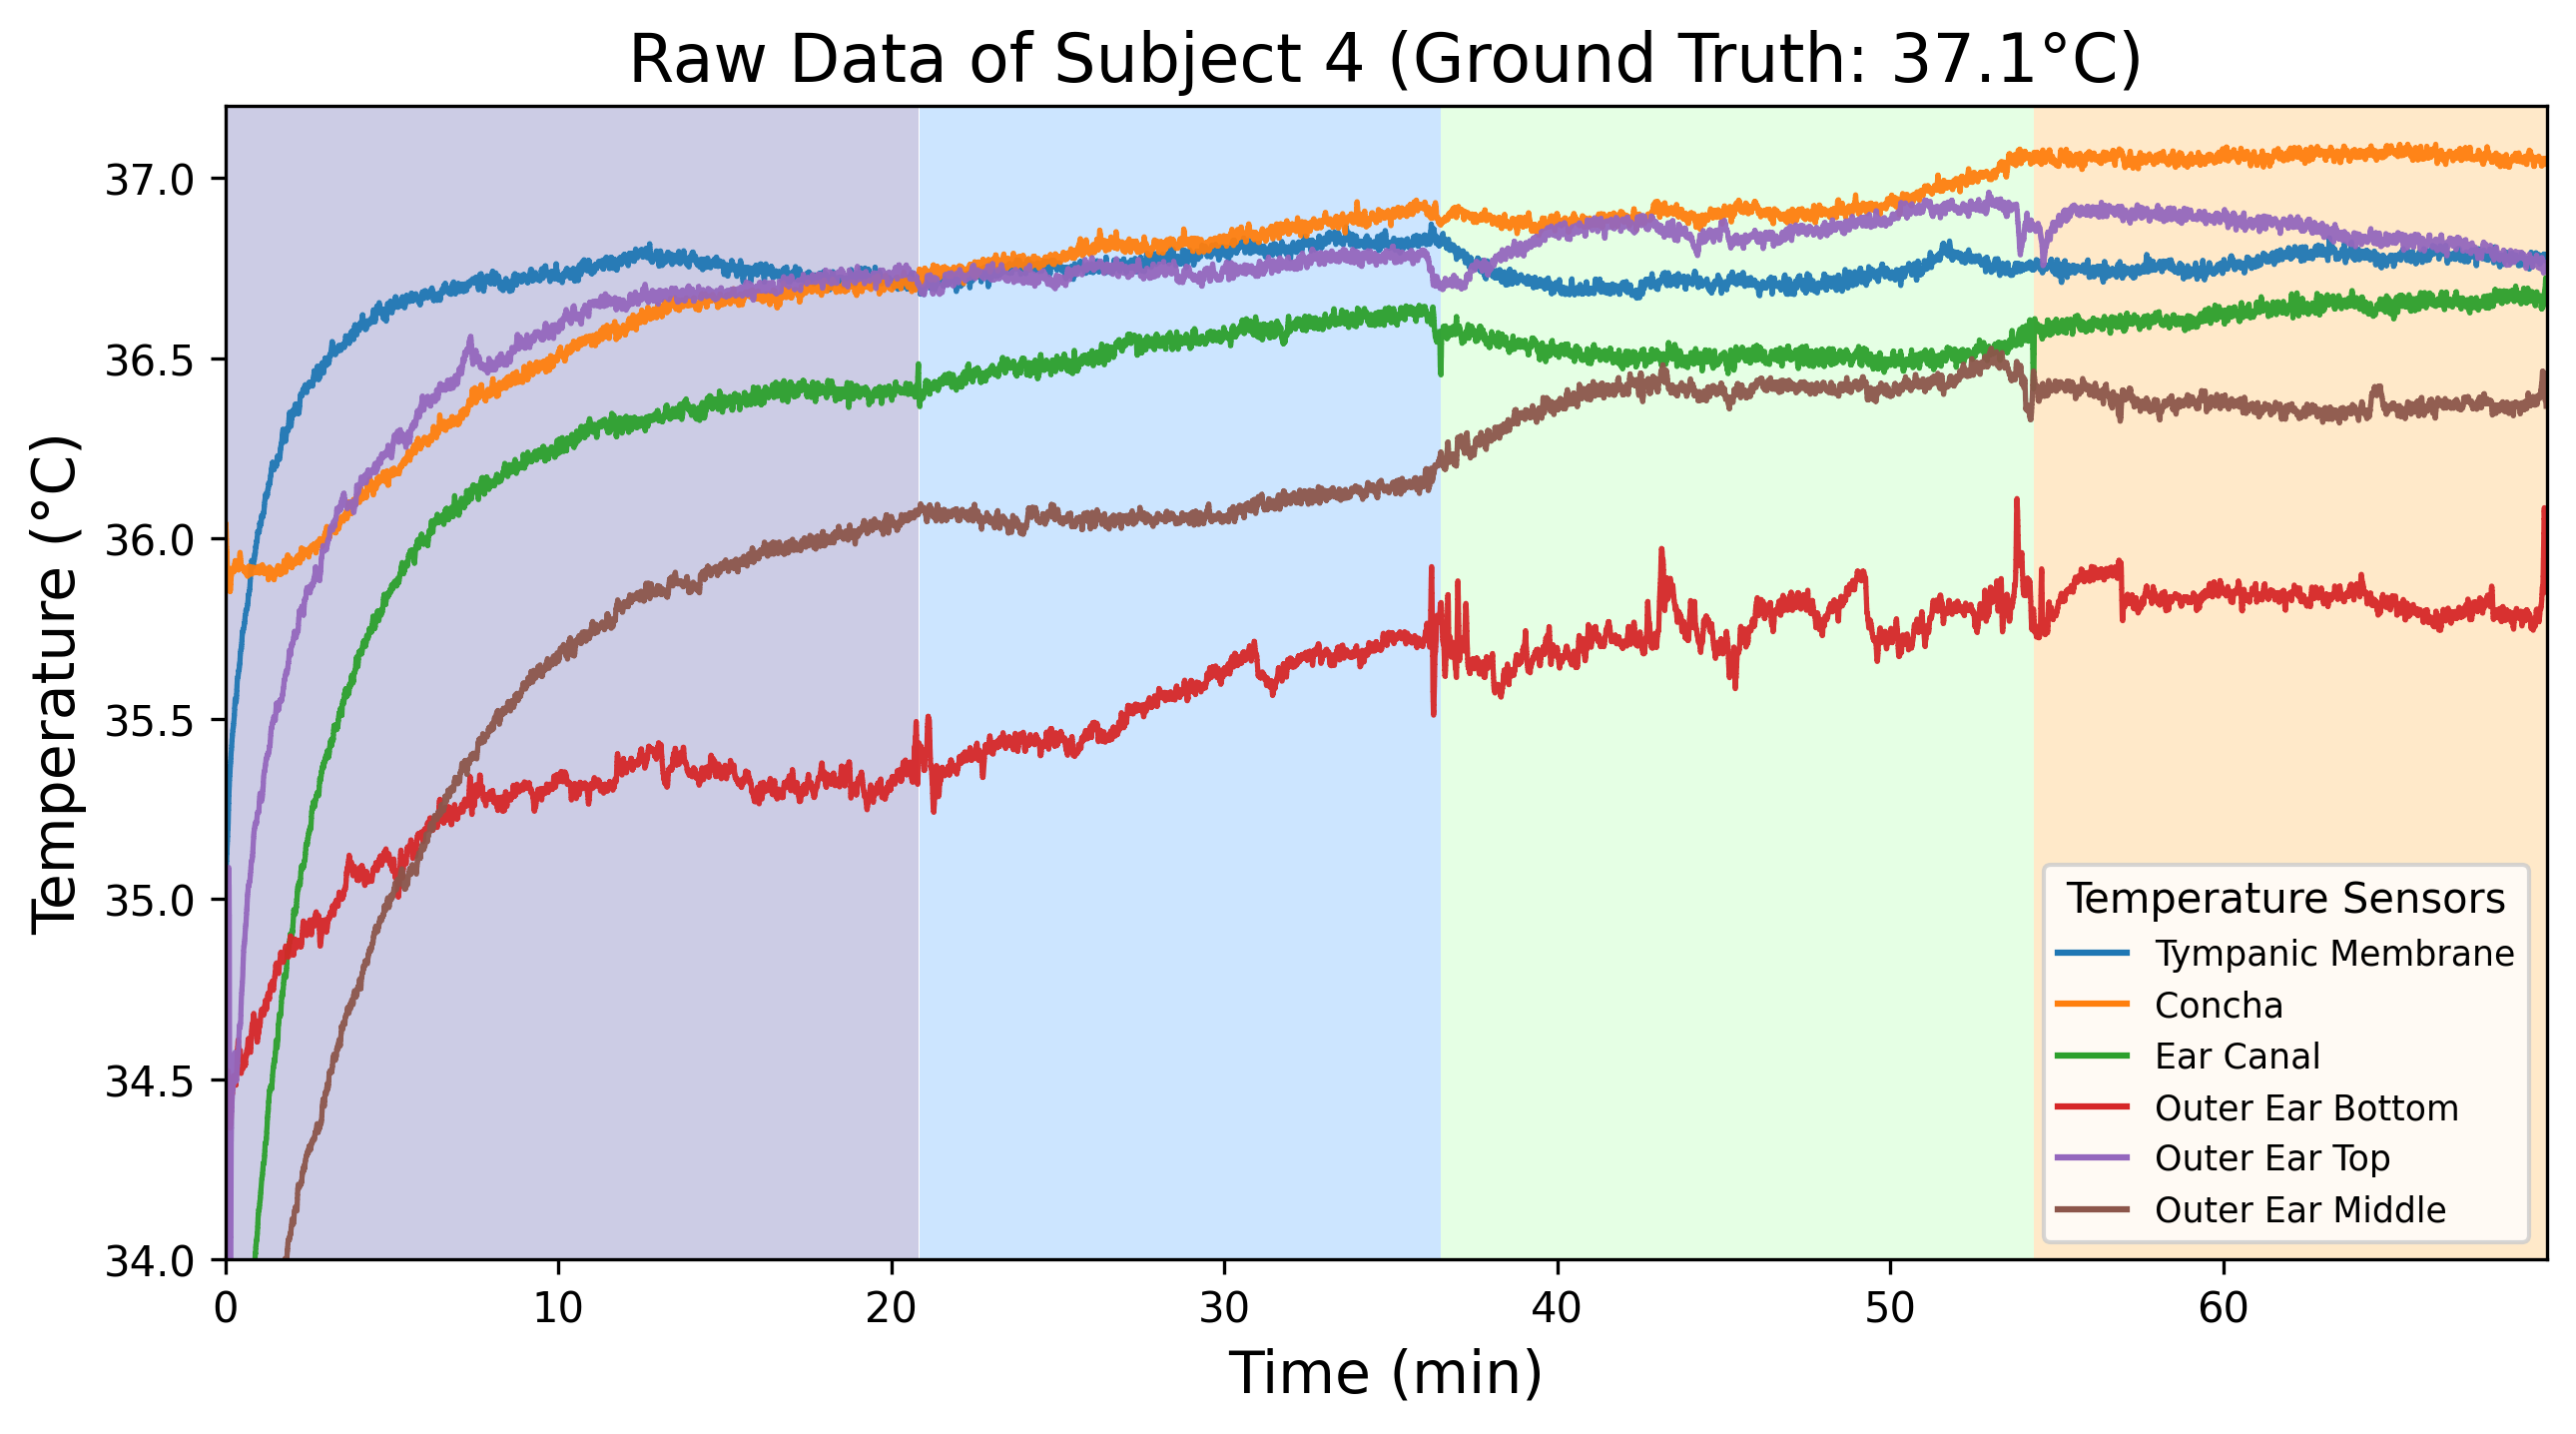
\includegraphics[width=\textwidth]{thesis-doc/images/study2/p04/Logging_study2_p04_0smoothed_raw_data.png}
    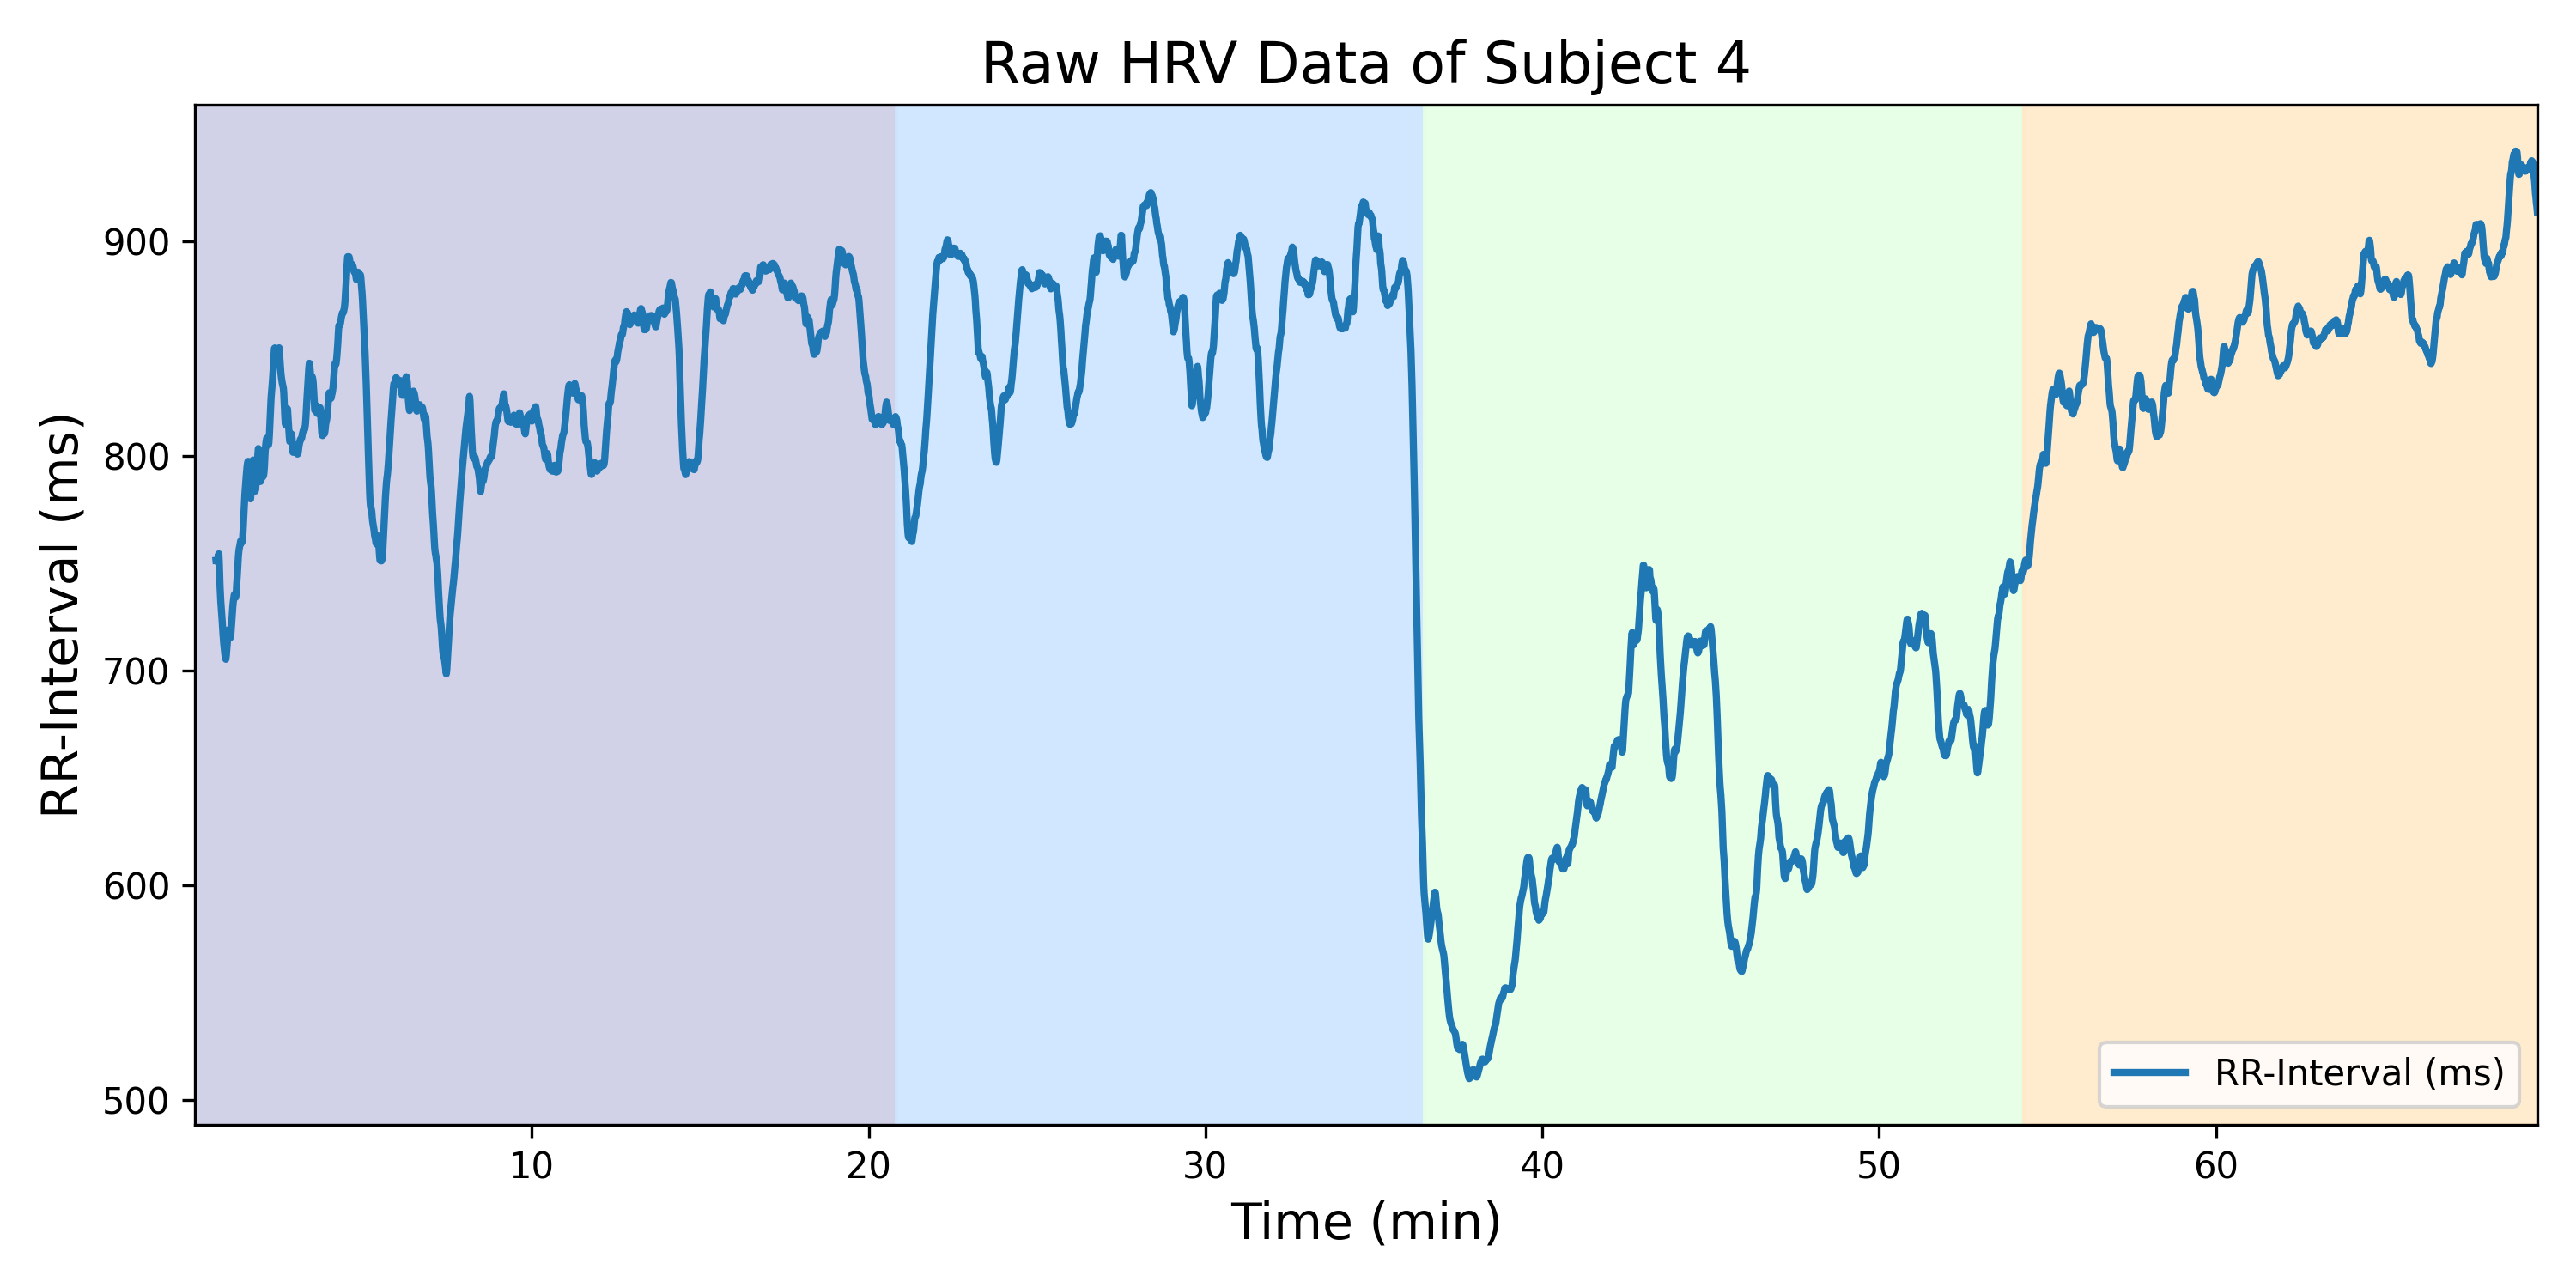
\includegraphics[width=\textwidth]{thesis-doc/images/study2/p04/raw_hrv_data_participant_4.png}
    \caption{Raw data from Subject 4 during the complete measurement. In the first phase (acclimatization phase), the sensors get used to the new environment. In Phase 2 the baseline was measured, in Phase 3 the test person was put under stress. Phase 4 represents the relaxation phase.}
    \label{fig:ch:Evaluation:Study2:RawData}
\end{figure}

\subsection{Stress Detection}
\label{subsec:Evaluation:Study2:ground_truth}
\begin{figure}[!t]
\begin{minipage}{\textwidth}
        \centering
        \resizebox{\textwidth}{!}{%
            \begin{tabularx}{1.2\textwidth}{|c|*{12}{>{\centering\arraybackslash}X|}}
            \hline
            \textbf{Subj.} & \multicolumn{2}{c|}{\textbf{SDNN (ms)}} & \multicolumn{2}{c|}{\textbf{RMSSD (ms)}} & \multicolumn{2}{c|}{\textbf{LF/HF}} & \multicolumn{2}{c|}{\textbf{Stress-Index}} & \multicolumn{2}{c|}{\textbf{PNS Index}} & \multicolumn{2}{c|}{\textbf{SNS Index}} \\
             & \textbf{Base} & \textbf{Stress} & \textbf{Base} & \textbf{Stress} & \textbf{Base} & \textbf{Stress} & \textbf{Base} & \textbf{Stress} & \textbf{Base} & \textbf{Stress} & \textbf{Base} & \textbf{Stress} \\
            \hline
            1 & 65.89 & 47.25 & 29.66 & 21.99 & 12.08 & 9.80 & 7 & 11 & -1.6 & -1.85 & 1.96 & 2.73 \\
        2 & 70.93 & 71.62 & 42.05 & 44.76 & 2.75 & 3.49 & 8 & 8 & -0.92 & -0.98 & 0.87 & 1.02 \\
        3 & 150.45 & 163.09 & 99.82 & 79.58 & 0.68 & 1.22 & 5 & 6 & 2.21 & 0.92 & -1.33 & -0.51 \\
        4 & 101.44 & 71.71 & 35.86 & 19.37 & 2.08 & 4.40 & 9 & 14 & -0.51 & -2.01 & 0.33 & 2.73 \\
        5 & 225.16 & 202.75 & 268.12 & 235.46 & 0.29 & 0.34 & 2 & 2 & 7.26 & 6.44 & -2.28 & -2.24 \\
            \hline
            \end{tabularx}
        }
    \end{minipage}
    \vspace{2em}  % Adds vertical space
    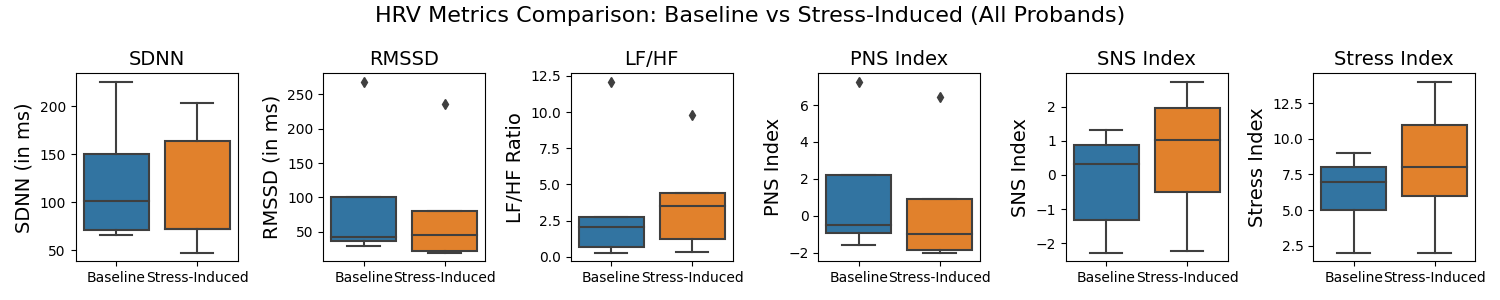
\includegraphics[width=\textwidth]{thesis-doc/images/study2/hrv_metrics_comparison.png}
    \vspace{2em}  % Adds vertical space
    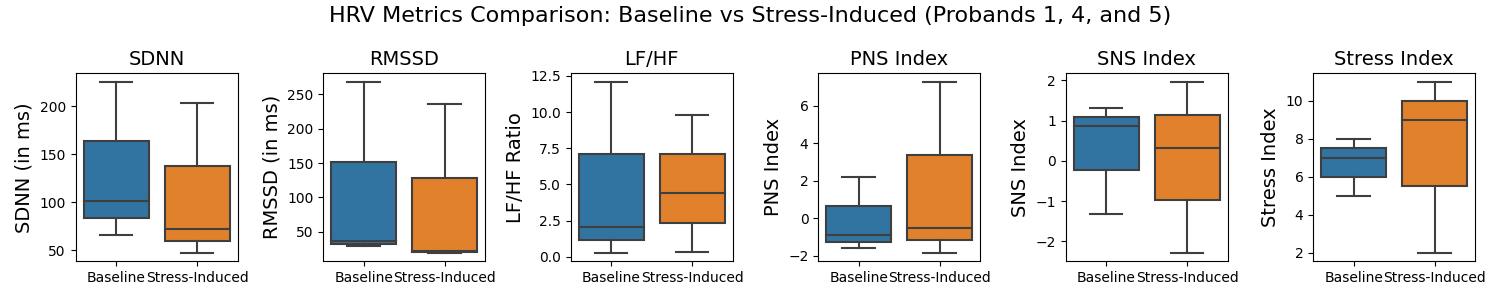
\includegraphics[width=\textwidth]{thesis-doc/images/study2/hrv_metrics_comparison_145.png}
    \caption{Comparison of heart rate variability (HRV) between baseline and stress induced phase in five subjects. SDNN, RMSSD, and LF/HF are HRV metrics, while stress index, PNS index, and SNS index are derived from analysis using "KubiosHRV Standard" software. All metrics are presented as pairs, with the baseline value appearing first, followed by the value under stress-induced conditions. Additionally, the values are presented as a boxplot across all subjects. The PNS is the regeneration index and indicates the recovery ability. The lower the value, the higher the regeneration phase and the more stressed the person is. The normal value is 0. The SNS is the stress index. The higher this value is, the higher the stress and accordingly the more stressed the person is. Here, too, the normal value is 0.}
    \label{subsec:Evaluation:Study2:ground_truth_result}
\end{figure}


At the outset, we examine whether the study actually produced stress in the subjects. 
This is necessary because the stress detection procedures used, although scientifically accepted, do not produce good results in every subject. 
A much better stress test would be the Trier Social Stress Test (TSST), but the time effort for such a huge study was not possible for this master thesis. 
To verify the stress score, HRV (heart rate variability) values were recorded using the Polar H9.
These are saved in the form of a txt file, in which the RR intervals (resting rate) were persisted.
With this information all values needed for the classification of stress can be calculated.
These include SDNN (Standard Deviation of NN intervals), RMSSD (Root Mean Square of Successive Differences) and LF/HF (Low Frequency/High Frequency).
The SDNN represents the variability in the time between successive heartbeats (NN intervals). 
Higher SDNN often indicates better autonomic flexibility, although it may increase or decrease under stress depending on individual variability.
The RMSSD is another HRV metric for the classification of short-term variations in heart rate.
In general, higher RMSSD values represent a healthier heart and lower stress.
However, this can vary from person to person.
The LF/HF ratio is a widely used analysis method to describe the balance between parasympathetic and sympathetic activities. 
Higher values often describe the dominance of sympathetic activity, i.e. stress. 
Lower values rather describe the dominance of the parasympathetic activity, i.e. relaxation.
In addition, other measures were considered using the "KubiusHRV Standard" software.
The software provides the parameters SNS index (Sympathetic Nervous System), PNS index (Parasympathetic Nervous System) and a stress index, which should confirm the findings from SDNN, RMSSD and LF/HF ratio.
The SNS index describes the activities of the sympathetic nervous system. 
Higher positive values induce stress or fight-or-flight responses.
The PNS index describes the activities of the parasympathetic nervous system. 
Higher positive values indicate relaxation.
The results are shown in Figure \ref{subsec:Evaluation:Study2:ground_truth_result}. 

Here it can be seen that for Subject 1, the SDNN and RMSSD value decreased during the stress-induced phase, which is an indication of stress.
However, for Subject 1 there is also a decrease in LF/HF ratio, which is contrary to a normal stress-induced phase.
The two SNS and PNS indices are helpful here, as values indicate stress, as the stress index does, which increases from 7 to 11.
For Test Person 2, a slight increase in the values can be seen in the stress-induced phase, which is contrary to the expectation of recognizing stress.
The stress index also remains stable at the value 8, which confirms the values. 
The PNS and SNS indices show slight increases, which could indicate stress, but the increases are not sufficient to detect a stronger tendency here. 
Test Person 3, no stress can be detected on the basis of the SDNN and RMSSD values either, as an increase in the SDNN and a decrease in the RMSSD values can be seen here. 
However, the LF/HF ratio increases, which indicates stress, as the slight decrease in the PNS index and slight increase in the stress index to 14. 
However, the decrease in the SNS index is an atypical sign of stress, which is why stress cannot be accurately attributed to Subject 3 either.
Proband 4 delivers the best values.
Here a significant decrease of the SDNN and RMSSD values during the stress-induced phase, a dramatic increase of the LF/HF ratio, a strongly increasing stress index to 14.
Furthermored, changes of PNS and SNS indices can be seen, which are all clear indications for stress.
Subject 4 here provides exactly the expected responses to stress.
Subject 5, on the other hand, shows a decrease in SDNN and RMSSD during the stress-induced phase. 
This indicates stress, which is confirmed by the slight increase in the LF/HF ratio.
However, the stress index remained stable for Subject 5, and the PNS and SNS index increased slightly, which is additionally indicative of stress, even though the increases are very small.

In summary, the study showed mixed efficacy in eliciting stress in the subjects, with Subject 4 showing the most consistent and significant signs of stress across all measurements. Interestingly, the male subjects (1, 4, and 5) generally showed more significant signs of stress compared to the female subjects (2 and 3) who showed ambiguous or inconsistent signs. This suggests that gender plays a role in these physiological responses, although further studies would be needed to confirm this hypothesis.
However, this statement should be taken with extreme caution, as such conclusions are very difficult to make with such a small number of subjects.
However, there is a tendency which can be further investigated by further studies.

\subsection{Hypothesis 1: Stress-Induced Temperature Rise}
\label{subsec:Evaluation:Study2:Hypothesis1}

\begin{figure}[t]
    \centering
    
    \begin{subtable}{\textwidth}
        \centering
        \begin{tabular}{|l|rrrrrr|}
        \hline
        \textbf{Subject} & \textbf{Tympanic} & \textbf{Concha} & \textbf{EarCanal} & \textbf{Outer Ear} & \textbf{Outer Ear} & \textbf{Outer Ear} \\
             & \textbf{Membrane} &  &  & \textbf{Bottom} & \textbf{Top} & \textbf{Middle} \\   
             &\textbf{(in \(^\circ\text{C}\))} & \textbf{(in \(^\circ\text{C}\))} & \textbf{(in \(^\circ\text{C}\))} & \textbf{(in \(^\circ\text{C}\))} & \textbf{(in \(^\circ\text{C}\))} & \textbf{(in \(^\circ\text{C}\))} \\
        \hline
        1 & -0.04 & -0.0 & -0.08 & 0.25 & 0.11 & 0.19 \\
        2 & -0.01 & 0.2 & 0.16 & 0.14 & 0.1 & 0.27 \\
        3 & 0.0 & 0.21 & 0.17 & 0.15 & 0.12 & 0.02 \\
        4 & -0.05 & 0.1 & -0.02 & 0.2 & 0.11 & 0.32 \\
        5 & -0.04 & 0.0 & -0.04 & 0.05 & 0.03 & 0.11 \\
        \hline
        \end{tabular}
        \caption{Temperature Difference from Baseline to Stress for each participant.}
        \label{subsec:Evaluation:Study2:Hypothesis1:temp_diff_sitting_to_stress_all}
    \end{subtable}
    
    \vspace{1em} % Add some vertical spacing between the tables
    
    \begin{subtable}{\textwidth}
        \centering
        \begin{tabular}{|l|rrrrrr|}
        \hline
        \textbf{Subject} & \textbf{Tympanic} & \textbf{Concha} & \textbf{EarCanal} & \textbf{Outer Ear} & \textbf{Outer Ear} & \textbf{Outer Ear} \\
             & \textbf{Membrane} &  &  & \textbf{Bottom} & \textbf{Top} & \textbf{Middle} \\   
             &\textbf{(in \(^\circ\text{C}\))} & \textbf{(in \(^\circ\text{C}\))} & \textbf{(in \(^\circ\text{C}\))} & \textbf{(in \(^\circ\text{C}\))} & \textbf{(in \(^\circ\text{C}\))} & \textbf{(in \(^\circ\text{C}\))} \\
        \hline
        1 & -0.02 & -0.08 & -0.07 & -0.15 & -0.04 & -0.04 \\
        2 & 0.0 & 0.14 & 0.16 & 0.07 & 0.04 & 0.14 \\
        3 & -0.03 & 0.1 & 0.11 & 0.28 & 0.02 & 0.11 \\
        4 & 0.04 & 0.14 & 0.12 & 0.08 & 0.0 & -0.02 \\
        5 & -0.15 & -0.12 & -0.13 & -0.11 & -0.06 & -0.07 \\
        \hline
        \end{tabular}
        \caption{Temperature Difference from stress-induced to relaxation for each participant.}
        \label{subsec:Evaluation:Study2:Hypothesis1:temp_diff_stress_to_relax_all}
    \end{subtable} 
    \caption{Evaluation of Hypotheses 1: Mean temperature changes during baseline, stress-induced, and relaxation phases. The tables represent the temperature changes between the phases. A negative value implies a temperature fall between the two comparing phases, and a positive value implies a temperature rise, respectively.}
    \label{sec:Evaluation:Study2:Hypothesis1:Summary}
\end{figure}

To evaluate hypothesis 1, the analysis focuses on the average temperature changes measured by different ear-based sensors during three different phases: baseline, stress-induced, and relaxation. 
The first phase, which serves to acclimate the temperature sensors, is disregarded here for analysis.
To ensure a fair comparison, the mean temperatures were subtracted with the ground truth for each participant.

To evaluate the hypothesis, the mean temperature per sensor per subject is calculated.
From this, the temperature differences of the different phases are calculated, which can be seen in Figure \ref{sec:Evaluation:Study2:Hypothesis1:Summary}.
Here, table \ref{subsec:Evaluation:Study2:Hypothesis1:temp_diff_sitting_to_stress_all} shows the mean temperature difference between the baseline and stress-induced phases, and table \ref{subsec:Evaluation:Study2:Hypothesis1:temp_diff_stress_to_relax_all} between the stress-induced and relaxation phases.
A significant increase of up to $0.6 ^\circ C$ can be expected \cite{vinkersEffectStressCore2013, okaMechanismsMediatorsPsychological2001, marksNonshiveringThermogenesisInterscapular2009}.
The largest increase in temperature to the stress-induced phase is observed behind the ear in the middle with $0.27 ^\circ C$, however, these results are not consistent enough. 
Most importantly, they are not consistent with the additional assumption that the temperature of the tympanic membrane provides the most accurate measurement results.
This records a temperature drop of $-0.04 ^\circ C$.
In summary, the data do not provide clear evidence for the hypothesis. 
While there are minor variations, they are not consistently in the direction of a temperature increase during the stress-induced phase, making it difficult to definitively confirm the hypothesis. 
It is important to note at this point that the conduct of the study is also a critical factor. 
Since the study was conducted in a short time frame that did not allow for a social stress test (TSST) to be conducted, and also only five subjects were used in the study, a re-study with a larger sample is recommended to reach a more conclusive conclusion.

\subsection{Hypothesis 2: Stress Test Temperature Variability}
\label{subsec:Evaluation:Study2:Hypothesis2}
Hypothesis 2 states that the temperature changes between the different stress tests. 
This can happen because stress is triggered by the sympathetic nervous system when the body goes into fight-or-flight mode.
This may be addressed differently during the different stress tests, which is then reflected in the body temperature.
To evaluate hypothesis 2, the mean temperature change between each stress test per subject is calculated.
The results are shown in Figure \ref{sec:Evaluation:Study2:Hypothesis2:Summary}. 
Here, Table \ref{subsec:Evaluation:Study2:Hypothesis2:temp_diff_stroop_nback} shows the mean temperature differences between the Stroop test and the N-back test, Table \ref{subsec:Evaluation:Study2:Hypothesis2:temp_diff_nback_math} between the N-back test and the math test.
The results show that there is no measurable temperature difference between the tests.
Since previous studies have already shown that the signal at the tympanic membrane is the most accurate, no pattern is apparent with this small sample size.
In both comparisons of the two tables, the maximum temperature change is 0.16 $ ^\circ C$, which is definitely not due to a stress-induced temperature increase.

% \begin{figure}[!t]
%     \centering
%     % First Table: Mean Temperatures
%     \begin{subtable}{\textwidth}
%         \centering
%         \begin{tabularx}{\textwidth}{|l|*{6}{>{\centering\arraybackslash}X|}}
%         \hline
%         & \multicolumn{2}{c|}{\textbf{Stroop Test}} & \multicolumn{2}{c|}{\textbf{N-Back Test}} & \multicolumn{2}{c|}{\textbf{Math Test}} \\
%         & \textbf{All} & \textbf{1,4,5} & \textbf{All} & \textbf{1,4,5} & \textbf{All} & \textbf{1,4,5} \\
%         \textbf{Sensor} & \textbf{(in $^\circ \text{C}$)} & \textbf{(in $^\circ \text{C}$)} & \textbf{(in $^\circ \text{C}$)} & \textbf{(in $^\circ \text{C}$)} & \textbf{(in $^\circ \text{C}$)} & \textbf{(in $^\circ \text{C}$)} \\
%         \hline
%         \textbf{TympanicMembrane} & 0.06 & 0.15 & 0.03 & 0.12 & 0.02 & 0.09 \\
%         \textbf{Concha} & -0.53 & 0.0 & -0.5 & 0.02 & -0.46 & 0.01 \\
%         \textbf{EarCanal} & -0.4 & -0.07 & -0.42 & -0.1 & -0.4 & -0.14 \\
%         \textbf{Outer Ear Bottom} & -0.9 & -0.63 & -0.84 & -0.57 & -0.79 & -0.52 \\
%         \textbf{Outer Ear Top} & -0.43 & -0.25 & -0.37 & -0.19 & -0.33 & -0.18 \\
%         \textbf{Outer Ear Middle} & -0.71 & -0.55 & -0.63 & -0.47 & -0.56 & -0.44 \\
%         \hline
%         \end{tabularx}
%         \caption{Mean Temperature of each stress test over all participants and over participants 1,4, and 5. The measured ground truth values are subtracted from each participant's temperature data to combine the results in a more fair way.}
%         \label{subsec:Evaluation:Study2:Hypothesis2:combined_mean_temps}
%     \end{subtable}

%     \vspace{1em} % Add some vertical spacing between the tables

%     % Second Table: T-Tests
%     \begin{subtable}{\textwidth}
%     \centering
%     \resizebox{\textwidth}{!}{%
%     \begin{tabularx}{\textwidth}{|l|*{4}{>{\centering\arraybackslash}X|}}
%     \hline
%     \textbf{Sensor} & \multicolumn{2}{c|}{\textbf{Stroop-N-Back}} & \multicolumn{2}{c|}{\textbf{N-Back-Math}} \\
    
%     & \textbf{All} & \textbf{1,4,5} & \textbf{All} & \textbf{1,4,5} \\
    
%     & \textbf{p-value} & \textbf{p-value} & \textbf{p-value} & \textbf{p-value} \\
%     \hline
%     \textbf{Tympanic Membrane} & 0.20 & 0.32 & 0.47 & 0.43 \\
%     \textbf{Concha} & 0.06 & 0.34 & 0.25 & 0.86 \\
%     \textbf{Ear Canal} & 0.19 & 0.15 & 0.68 & 0.12 \\
%     \textbf{Outer Ear Bottom} & 0.004 & 0.064 & 0.047 & 0.055 \\
%     \textbf{Outer Ear Top} & 0.06 & 0.13 & 0.15 & 0.36 \\
%     \textbf{Outer Ear Middle} & 0.033 & 0.21 & 0.046 & 0.077 \\
%     \hline
% \end{tabularx}%
%     }
%     \caption{T-Test results for different sensors across phases for all subjects and for subjects 1,4,5. The p-value for transitions between Sitting - Stress and Stress - Relax are presented.}
%     \label{subsec:Evaluation:Study2:Hypothesis1:TTest_Results}
% \end{subtable}
    
%     \caption{Evaluation results of Hypothesis 2 including Mean temperatures in the Stroop, N-Back, and Math tests with all subjects and additionally subjects 1, 4 and 5, as only these showed stress responses in Ground Truth. For this purpose, the results of the significance test are listed to show their significance.}
%     \label{sec:Evaluation:Study2:Hypothesis2:Summary}
% \end{figure}
\begin{figure}[!t]
    \centering
    % First Table: Mean Temperatures
    \begin{subtable}{\textwidth}
        \centering
        \resizebox{\textwidth}{!}{%
            \begin{tabular}{|l|rrrrrr|}
            \hline
            \textbf{Subject} & \textbf{Tympanic} & \textbf{Concha} & \textbf{EarCanal} & \textbf{Outer Ear} & \textbf{Outer Ear} & \textbf{Outer Ear} \\
             & \textbf{Membrane} &  &  & \textbf{Bottom} & \textbf{Top} & \textbf{Middle} \\   
             &\textbf{(in \(^\circ\text{C}\))} & \textbf{(in \(^\circ\text{C}\))} & \textbf{(in \(^\circ\text{C}\))} & \textbf{(in \(^\circ\text{C}\))} & \textbf{(in \(^\circ\text{C}\))} & \textbf{(in \(^\circ\text{C}\))} \\
            \hline
            1 & 0.0 & 0.03 & -0.02 & 0.05 & 0.03 & 0.02 \\
            2 & -0.01 & 0.06 & -0.03 & 0.07 & -0.01 & 0.11 \\
            3 & -0.01 & 0.05 & 0.02 & 0.04 & 0.09 & 0.05 \\
            4 & -0.08 & -0.01 & -0.06 & 0.04 & 0.11 & 0.16 \\
            5 & -0.02 & 0.03 & -0.02 & 0.09 & 0.05 & 0.06 \\
            \hline
            \end{tabular}
        }
        \caption{Temperature differences between Stroop and N-Back for each participant.}
        \label{subsec:Evaluation:Study2:Hypothesis2:temp_diff_stroop_nback}
    \end{subtable}

    \vspace{1em} % Add some vertical spacing between the tables

    % Second Table: T-Tests
    \begin{subtable}{\textwidth}
        \centering
        \resizebox{\textwidth}{!}{%
            \begin{tabular}{|l|rrrrrr|}
            \hline
            \textbf{Subject} & \textbf{Tympanic} & \textbf{Concha} & \textbf{EarCanal} & \textbf{Outer Ear} & \textbf{Outer Ear} & \textbf{Outer Ear} \\
             & \textbf{Membrane} &  &  & \textbf{Bottom} & \textbf{Top} & \textbf{Middle} \\   
             &\textbf{(in \(^\circ\text{C}\))} & \textbf{(in \(^\circ\text{C}\))} & \textbf{(in \(^\circ\text{C}\))} & \textbf{(in \(^\circ\text{C}\))} & \textbf{(in \(^\circ\text{C}\))} & \textbf{(in \(^\circ\text{C}\))} \\
            \hline
            1 & -0.06 & -0.01 & -0.05 & 0.03 & 0.02 & 0.05 \\
            2 & -0.03 & 0.09 & 0.1 & 0.0 & 0.05 & 0.11 \\
            3 & 0.03 & 0.12 & 0.11 & 0.1 & 0.13 & 0.13 \\
            4 & 0.02 & 0.03 & -0.01 & 0.06 & 0.01 & 0.02 \\
            5 & -0.03 & -0.04 & -0.07 & 0.07 & -0.01 & 0.02 \\
            \hline
            \end{tabular}
        }
        \caption{Temperature differences between N-Back and Math for each participant.}
        \label{subsec:Evaluation:Study2:Hypothesis2:temp_diff_nback_math}
    \end{subtable}
    
    \caption{Summary of Hypothesis 2 Evaluation. The tables show mean temperature differences in \(^\circ\text{C}\) for subjects participating in Stroop, N-Back, and Math stress tests between the different stress tests. A negative value implies a temperature fall between the two comparing phases, and a positive value implies a temperature rise, respectively.}

    \label{sec:Evaluation:Study2:Hypothesis2:Summary}
\end{figure}

In summary, hypothesis 2 assumed that temperature changes between different stress tests would be detectable due to different sympathetic nervous system responses. However, the analysis as detailed in Figure \ref{sec:Evaluation:Study2:Hypothesis2:Summary} does not support this hypothesis. In particular, the tympanic membrane, previously identified as the most reliable sensor, showed negligible temperature changes during the stress tests. With a maximum temperature shift of $0.16 ^\circ C$, the observed variations are statistically insignificant and cannot be attributed to stress-induced temperature changes. This limitation may be due in part to the small sample size, suggesting that more comprehensive studies are needed for a conclusive evaluation.
In addition, a Trier Social Stress Test (TSST) could induce a stronger stress condition.

\subsection{Further Discussion}
For Study 2, there are additional hypotheses that can be considered. 
First, the correlation between heart rate variability (HRV) and ear temperature can be considered. 
In addition, it can be considered whether the ear temperature returns to the "normal level" after the stress-induced phase.
It can also be considered that the regeneration of the body after the stress test differs from subject to subject and takes different amounts of time to return to baseline temperature.
In addition, the thesis can be considered that stress has different characteristics between male and female subjects and whether this is also reflected in the temperature.
For this, however, the number of subjects must be significantly higher.
However, it can already be seen in Table \ref{sec:Evaluation:Study2:Hypothesis1:Summary} that the temperature hardly changes between the stress-induced phase and the phases around it. 
Because of this, the analyses are not continued here, as a new study with an increased number of subjects is needed.
In addition, the selected stress tests (as already mentioned in Section \ref{ch:Design:Study:Study1}) do not elicit sufficient stress in every subject.
A Trier social stress test (TSST) is also a clearly scientifically recognized stress test, which should be considered for this purpose in the future.
In summary, Study 2 has provided very helpful information and some approaches for future work, but no meaningful conclusions can be confirmed.